\documentclass[10pt,a4paper]{article}

\usepackage[utf8]{inputenc}		% Configuro la codificación
\input{.command.tex}
% En el siguiente archivo se configuran las variables del trabajo práctico
%% \providecommand es similar a \newcommnad, salvo que el primero ante un 
%% conflicto en la compilación, es ignorado.

% Al comienzo de un TP se debe modificar los argumentos de los comandos

\providecommand{\myTitle}{TRABAJO PRÁCTICO 2} 
\providecommand{\mySubtitle}{Filtro de Kalman}

\providecommand{\mySubject}{Procesamiento de Señales II (86.52)}
\providecommand{\myKeywords}{UBA, Ingeniería, PS2}

\providecommand{\myAuthorSurname}{Manso}
\providecommand{\myTimePeriod}{Año 2018 - 2\textsuperscript{do} Cuatrimestre}

% No es necesario modificar este %%%%%%%%%%%%%%
\providecommand{\myHeaderLogo}{header_fiuba}
%%%%%%%%%%%%%%%%%%%%%%%%%%%%%%%%%%%%%%%%%%%%%%%%

% Si se utilizan listings, definir el lenguaje aquí
\providecommand{\myLanguage}{matlab} 
% Crear los integrantes del TP con el comando \PutMember donde
%%		1) Apellido, Nombre
%%		2) Número de Padrón
%%		3) E-Mail
\providecommand{\MembersOnCover}[0]
{		
		\PutMember{Anastópulos, Matías}{95120}{matias.anas@gmail.com}
		\PutMember{Gasparovic, Emiliano}{96123}{emilianit2000@gmail.com}
		\PutMember{Manso, Juan} {96133} {juanmanso@gmail.com}
}

\providecommand{\myGroupNumber}{02}


\Pagebreaktrue		% Setea si hay un salto de página en la carátula
\Indextrue
\Siunitxtrue			% Si quiero utilizar el paquete, \siunixtrue. Si no \siunixfalse
\Todonotestrue		% Habilita/Deshabilita las To-Do Notes y las funciones \unsure, \change, \info, \improvement y \thiswillnotshow.
\Listingstrue
\Keywordsfalse
\Putgrouptrue		% Habilita/Deshabilita el \myGroup en los headers
\Videofalse
				% Archivo con los comandos globales como Título y autores
%Preambulo para articulo científico de LaTeX

\usepackage[a4paper,left=3cm,right=3cm,bottom=3.5cm,top=3.5cm]{geometry} 	% Configuro la geometría del papel
%\usepackage{microtype}								% Mejora el "spacing" de las palabras
\usepackage[spanish]{babel} 							% Compatibilizo los signos del español
	\addto\captionsspanish{\renewcommand{\tablename}{Tabla}}		%% Redefino nombres preestablecidos por Babel
	\addto\captionsspanish{\renewcommand{\listtablename}{Índice de tablas}}	%% y así en vez de Cuadro dirá Tabla.
\usepackage{amsmath, amsfonts, amssymb}						% Entornos matemáticos, fuentes y símbolos
\usepackage{graphicx}								% Necesario para insertar figuras
\usepackage{fancyhdr}								% Para manipular headers y footers
\usepackage[usenames,dvipsnames]{color}						% \color{color deseado} {lo que querés que tenga color}
\usepackage{subcaption}								% Permite captions del tipo 1a, 1b
\usepackage{multirow}								% Para tablas
\usepackage{float}

% Para video
\ifVideo
	\usepackage{media9}
	\addmediapath{./../reportes/}
\fi

%\usepackage{times}
%\usepackage{mathtools}
%\usepackage{upgreek} % letras griegas sin cursiva
%\usepackage{cancel}
\usepackage{rotating}
\usepackage{tikz}
\usepackage{pgfplots}
%	\pgfplotsset{compat=1.12}
	\usetikzlibrary{plotmarks}% matlab2tikz
\usepackage{grffile}% matlab2tikz 
	\usetikzlibrary{calc,patterns,decorations.pathmorphing,decorations.markings}

\ifListings
	\usepackage{listings}

	\providecommand{\lstinputpath}[1]{\lstset{inputpath=#1}}

%	\input{.lst_default.tex}
	\input{.lst_matlab.tex}
%	\input{.lst_c.tex}
%	\input{.lst_c++.tex}
	
% 	\input{.lst_pseudocode.tex}


\fi

\ifSiunitx
\usepackage{siunitx}											% Unidades: \SI {cantidad} {\unidad} (necesita texlive-science)
	\sisetup{load-configurations = abbreviations}							% Habilita poner \cm en vez de \centi\metre
	\sisetup{output-decimal-marker = {,}}									% Cambia los puntos decimales por comas
	\sisetup{per-mode = fraction}											% Pone las unidades como fracción
	\sisetup{quotient-mode = fraction}										
\fi


\ifTodonotes
\usepackage{xargs}
\usepackage[colorinlistoftodos,prependcaption,textsize=tiny]{todonotes}


	\newcommandx{\Juan}[2][1=]{\todo[linecolor=blue,backgroundcolor=blue!25,bordercolor=blue,#1]{#2}}
	\newcommandx{\Mati}[2][1=]{\todo[linecolor=green,backgroundcolor=green!25,bordercolor=green,#1]{#2}} % OliveGreen
	\newcommandx{\Emi}[2][1=]{\todo[linecolor=Plum,backgroundcolor=Plum!25,bordercolor=Plum,#1]{#2}}
	\newcommandx{\unsure}[2][1=]{\todo[linecolor=red,backgroundcolor=red!25,bordercolor=red,#1]{#2}}
	\newcommandx{\thiswillnotshow}[2][1=]{\todo[disable,#1]{#2}}
\fi


\usepackage{booktabs}														% Permite hacer tablas sin separadores en el medio
\usepackage{placeins}														
		\let\Oldsection\section												%% Permite que los flotantes (como figuras) no aparescan
	\renewcommand{\section}{\FloatBarrier\Oldsection}						%% antes o después de su sección correspondiente.
		\let\Oldsubsection\subsection
	\renewcommand{\subsection}{\FloatBarrier\Oldsubsection}		
		\let\Oldsubsubsection\subsubsection
	\renewcommand{\subsubsection}{\FloatBarrier\Oldsubsubsection}
\usepackage{hyperref}														% Debe ser agregado al final del preambulo

\hypersetup
{    bookmarks=true,         % show bookmarks bar?
     unicode=false,          % non-Latin characters in Acrobat’s bookmarks
     pdftoolbar=true,        % show Acrobat’s toolbar?
     pdfmenubar=true,        % show Acrobat’s menu?
     pdffitwindow=false,     % window fit to page when opened
     pdftitle={\myTitle},    		 % title
     pdfauthor={\myAuthorSurname},   % author
	 pdfcreator={\myAuthorSurname},	 % creator = author
     pdfsubject={\mySubject},		 % subject of the document
     pdfkeywords={\myKeywords},
     colorlinks=true,        % false: boxed links; true: colored links
     linkcolor=black,        % color of internal links (change box color with linkbordercolor)
     citecolor=black,        % color of links to bibliography
     filecolor=magenta,      % color of file links
     urlcolor=cyan           % color of external links
}

%Configuro la pagina con los encabezaos y pies de paginas
\pagestyle{fancy}										% Para agregar encabezados y pie de paginas	
\lhead{\mySubject}										% Encabezado izquierdo
\rhead{\includegraphics[scale=0.15]{\myHeaderLogo}} 	% Encabezado derecho (logo de la FIUBA)	
\ifPutgroup
\chead{\texttt{Grupo Nº\myGroupNumber} }%\\ \textit{\footnotesize{\myTimePeriod}}}
\fi				

%% Este archivo contiene las funciones auxiliares para escribir en LaTeX
%% Dichas funciones resuelven la sintaxis de generar figuras, por ejemplo,
%% dejando el código más compacto y facilitando la corrección del mismo.



% Comando para graficar eps. 1er arg, escala. 2do, ruta. 3ro, caption. 4to, label.
\providecommand{\HgraficarEPS}[4]{
			\begin{figure}[h!]
				\centering
					\scalebox{#1}{\input{#2}}
					\caption{#3}
					\label{#4}
			\end{figure}

}

\providecommand{\HgraficarPNG}[4]{
			\begin{figure}[h!]
				\centering
					\includegraphics[scale=#1]{#2}
					\caption{#3}
					\label{#4}
			\end{figure}

}


% Comando para graficar eps en el lugar previsto.
\providecommand{\graficarEPS}[4]{
			\begin{figure}[h]
				\centering
					\scalebox{#1}{\input{#2}}
					\caption{#3}
					\label{#4}
			\end{figure}

}

\providecommand{\graficarPNG}[4]{
			\begin{figure}[h]
				\centering
					\includegraphics[scale=#1]{#2}
					\caption{#3}
					\label{#4}
			\end{figure}

}

\providecommand{\graficarPDF}[3]{
			\begin{figure}[h!]
				\centering
		\includegraphics[width=1.0\textwidth,keepaspectratio]{#1}
					\caption{#2}
					\label{#3}
			\end{figure}

}


\providecommand{\graficarPDFwide}[3]{
			\begin{figure}[h!]
				\centering
		\includegraphics[scale=0.5,trim={6,5cm 0 0 0}]{#1}
					\caption{#2}
					\label{#3}
			\end{figure}

}

\providecommand{\graficarPDFa}[4]{
			\begin{figure}[h!]
				\centering
				\includegraphics[scale=0.5,trim={#1}]{#2}
					\caption{#3}
					\label{#4}
			\end{figure}

}



\providecommand{\underuparrow}[2]{\underset{\underset{#2} \uparrow} #1 }

\providecommand{\cltext}[2]{\color{#1}{\huge{#2}}}

\providecommand{\cstext}[2]{\color{#1}{\large{#2}}}

\providecommand{\vect}[1]{\boldsymbol{#1}}
\providecommand{\dvect}[1]{\dot{\boldsymbol{#1}}}
\providecommand{\dd}{\mathrm{d}}
		% Se proveen un conjunto de funciones extras

% Defino el path de los includegraphics
\graphicspath{{./Figuras/}}		% Directorio que contiene los graficos

% Defino el path para los input de .tex y de .eps
\makeatletter
\def\input@path{{./Figuras/}{./Secciones/}{./Cover_page/}}
\makeatother

% Defino el path del listings
\ifListings
%% Cambiar el nombre de la carpeta si se utilizan Listings
	\lstinputpath{{../Octave/}}
\fi

\definecolor{myred}{rgb}{0.5,0,0}
\definecolor{mygreen}{rgb}{0,0.5,0}

\renewcommand{\thesubsection}{\thesection.\alph{subsection}}

\begin{document}
		% Carátula (formal o simple,_formal o _simple respectivamente) con Resumen
		% incluido e Índice (si es necesario configurar en config.tex) del informe
		\begin{titlepage}
	
		\thispagestyle{empty}

		\begin{center}
			
\includegraphics[scale=0.3]{fiuba}\\
			\large{\textsc{Universidad de Buenos Aires}}\\
			\large{\textsc{Facultad De Ingeniería}}\\
			\small{\myTimePeriod}
		\end{center}

		\vfill

		\begin{center}
			\Large{\underline{\textsc{\mySubject}}}
		\end{center}

		\vfill

		\begin{tabbing}
			\hspace{2cm}\=\+\myTitle\\
				TEMA: \mySubtitle\\
				FECHA: \today\\
			\\
				\MembersHeader
				\MembersOnCover	
		\end{tabbing}

		\begin{abstract}
			% Ejemplo de Resumen
%% MANTENER EL NOMBRE %%
	El presente trabajo tiene como objetivo utilizar el filtro de Kalman para estimación de trayectorias y analizar sus modificaciones ante diversas condiciones.

		\end{abstract}

	\ifKeywords
		\begin{center}
			\emph{Palabras Clave: \myKeywords}
		\end{center}
	\fi	

		\vfill
	
\end{titlepage}

\ifPagebreak
	\thispagestyle{empty}
	\ifIndex
		\tableofcontents
%		\listoffigures
%		\listoftables
	\fi

	\pagebreak
\fi


	\setcounter{page}{1}

\begin{center}{\Large{\textbf{Enunciado}}}\end{center}
		
	Se considera un vehículo que se desplaza definiendo una trayectoria tal que la posición en cada instante resulta $\vect{p}(t)$ y con una velocidad $\vect{v}(t)$, definidas en un plano de coordenadas inerciales $[x^e,y^e]$ de acuerdo a:
	\begin{equation*}
		\vect{p^e}(t) = \begin{bmatrix} p^e_x(t) \\[0.3em] p^e_y(t) \end{bmatrix} \qquad%
		\vect{v^e}(t) = \begin{bmatrix} v^e_x(t) \\[0.3em] v^e_y(t) \end{bmatrix}
	\end{equation*}

	\begin{equation}
		\begin{cases}
			\vect{\dot{p}^e}(t) = \vect{v^e}(t)\\
			\vect{\dot{v}^e}(t) = \vect{a^e}(t)\\
		\end{cases}
		\label{eq:din_inercial}
	\end{equation}

	Sin embargo, el dato de la aceleración viene dado en el sistema de coordenadas (terna que se denominará $b$) del vehículo que cambia su orientación a medida que se mueve. Por lo tanto, se define la variable $\theta(t)$ como se ve en la 
	\Juan{Generar e insertar figura de los ejes del avión}
	Figura \ref{fig:coordenadas_avion} que describe el ángulo de rotación del vehículo. El otro dato que se provee de la trayectoria es la velocidad angular $\omega(t) = \frac{\dd \theta}{\dd t} (t)$. En consecuencia, con todo lo enunciado previamente se plantean las ecuaciones de la dinámica del vehículo en \eqref{eq:din_veh}.

	\begin{equation}
		\begin{cases}
			\vect{\dot{p}^e}(t) = \vect{v^e}(t)\\[1.4em]
			\vect{\dot{v}^e}(t) = C^e_b \; \vect{a^b}(t)\\[0.6em]
			{C^e_b} = \dot{C}^e_b \; \begin{pmatrix} 0& -\omega(t)\\[0.3em] \omega(t)&0 \end{pmatrix}
		\end{cases}
		\label{eq:din_veh}
	\end{equation}

	donde $C^e_b = \begin{pmatrix} \cos(\theta(t)) & -\sen(\theta(t))\\[0.3em] \sen(\theta(t)) & \cos(\theta(t))\end{pmatrix}$






	\section{Modelo en variables de estado y filtro de Kalman}\label{sec:ej1}
			%\lstinputlisting[linerange=Hola-Chau]{../Informe/test.m}
	
	\Juan{Preguntar a Emi si podemos usar un \emph{approach} similar al otro tp o si está muy mal}
	Se define la variable de estado $\vect{x}(t)$ asociada al sistema como:
		\begin{equation*}
			\vect{x}(t) = \begin{bmatrix} {p_x}(t) \\[0.3em] p_y(t) \\[0.3em] {v_x}(t) \\[0.3em] v_y(t) \\[0.3em] c_{11}(t) \\[0.3em] c_{12}(t) \\[0.3em] c_{21}(t) \\[0.3em] c_{22}(t) \end{bmatrix} \qquad%
			\dot{\vect{x}}(t) = \begin{bmatrix} {\dot{p}_x}(t) \\[0.3em] \dot{p}_y(t) \\[0.3em] {\dot{v}_x}(t) \\[0.3em] \dot{v}_y(t) \\[0.3em] \dot{c}_{11}(t) \\[0.3em] \dot{c}_{12}(t) \\[0.3em] \dot{c}_{21}(t) \\[0.3em] \dot{c}_{22}(t) \end{bmatrix}
		\end{equation*}

	Así el modelo resulta:
		\begin{equation*}
			\Sigma:
			\begin{cases}
				\dvect{x}(t) = A\: \vect{x}(t) + B \: \vect{\xi}(t) \\
				\vect{y}(t) = C\: \vect{x}(t) + \vect{\eta}(t)
			\end{cases}
		\end{equation*}
	donde $\vect{\xi}(t)$ es el ruido de proceso y $\vect{\eta}(t)$ el ruido de medición. La matriz $A$ contiene la información de la dinámica del sistema, $B$ es la matriz de entrada del ruido de proceso, y la matriz de salida es $C$, que conecta los estados con las mediciones de posición y velocidad. Las matrices quedan caracterizadas por la ecuación \eqref{eq:matrix_cont}.
		\begin{equation}
			\label{eq:matrix_cont}
			A(t) = \begin{pmatrix}0&0&I&0&0&0&0&0\\[0.3em]0&0&0&I&0&0&0&0\\[0.3em]0&0&0&0&a^b_x&a^b_y&0&0\\[0.3em]0&0&0&0&0&0&a^b_x&a^b_y&\\[0.3em]0&0&0&0&0&\omega^b&0&0\\[0.3em]0&0&0&0&-\omega^b&0&0&0\\[0.3em]0&0&0&0&0&0&0&\omega^b\\[0.3em]0&0&0&0&0&0&-\omega^b&0\end{pmatrix} \quad%
			B = \begin{pmatrix}0&0&0\\[0.3em]0&0&0\\[0.3em]0&c_{11}&c_{12}\\[0.3em]0&c_{21}&c_{22}\\[0.3em]1&0&0\\[0.3em]-1&0&0\\[0.3em]1&0&0\\[0.3em]-1&0&0\end{pmatrix} \quad%
			C = \begin{pmatrix}I&0&0\\[0.3em]0&I&0\end{pmatrix}
		\end{equation}
	
	Para poder tratar el sistema en forma digital, es necesario definir un período de muestreo $T$, que en este caso es igual al periodo de muestreo del giróscopo \SI{100}{\Hz}. Así se tiene que la exponencial matricial es:
		\begin{equation*}
			e^{A\,t} \approx I + A\,T + \frac{(A\,T)^2}{2} + \hdots
		\end{equation*}

	Truncando a segundo orden y reemplazando por $A$ se obtiene:
		\begin{equation*}
			A_d = \begin{pmatrix}	I&0&T&0&a^b_x\:\frac{T^2}{2}&a^b_y\:\frac{T^2}{2}&0&0\\[0.3em]%
						0&I&0&T&0&0&a^b_x\:\frac{T^2}{2}&a^b_y\:\frac{T^2}{2}\\[0.3em]%
						0&0&I&0&a^b_x\:T-\:a^b_y\:\omega^b\:\frac{T^2}{2}&a^b_y\: T+a^b_x\:\omega^b\:\frac{T^2}{2}&0&0\\[0.3em]%
						0&0&0&I&0&0&a^b_x\:T-\:a^b_y\:\omega^b\:\frac{T^2}{2}&a^b_y\: T+a^b_x\:\omega^b\:\frac{T^2}{2}\\[0.3em]%
						0&0&0&0&I-\frac{(\omega\:T)^2}{2}&\omega\:T&0&0\\[0.3em]%
						0&0&0&0&-\omega\:T&I-\frac{(\omega\:T)^2}{2}&0&0\\[0.3em]%
						0&0&0&0&0&0&I-\frac{(\omega\:T)^2}{2}&\omega\:T\\[0.3em]%
						0&0&0&0&0&0&-\omega\:T&I-\frac{(\omega\:T)^2}{2}
		\end{pmatrix}
		\end{equation*}


		Con dicho modelo y las mediciones de posición, velocidad, aceleración no inercial y velocidad angular no inercial, se aplica el filtro de Kalman 
		\Juan{Qué opinan de éste final de oración?}
		donde se actualiza la matriz $A_d$ cada $T_s$ segundos y cada $100\, T_s$ llega la medición del radar haciendo posible la correción de los estados.
	
%
%	En cuanto a los ruidos, se hace la suposición que se tratan de ruidos blancos con matrices de covarianza $Q_{d}$ para el ruido de proceso y $R_{d}$ para el ruido de medición. Cabe aclarar que el hecho de que se trate de ruidos blancos no implica que $Q_{d}$ y $R_{d}$ sean diagonales. Ambas matrices dan información de la correlación componente a componente de los vectores de ruido.
%	

		
	\section{Estimación de la trayectoria}\label{sec:ej2}
		
\graficarPDF{graf_ej2}{Estimación de la trayectoria.}{fig:ej2}
	Al igual que en el trabajo práctico anterior, siendo todos los estados observables se obtiene una estimación muy buena de la trayectoria del vehículo como se expone en la Figura \ref{fig:ej2}. También se puede comprobar que el filtro de Kalman funciona correctamente al analizar las innovaciones (Figura \ref{fig:2covinn}). Se puede ver que la correlación de las mismas se asemeja al de un proceso blanco.
\graficarPDF{graf_ej2_covinn}{Innovaciones de las posiciones y velocidades en $x^e$ e $y^e$.}{fig:2covinn}
\graficarPDFa{0 0 8.0cm 8.0cm}{graf_ej2_pos}{Posición y error de la misma en función del tiempo.}{fig:2pos}
	\Juan{Checkear ésto}
	Examinando la posición en $x^e$ e $y^e$ se podría entender que la aproximación es buena. Sin embargo, analizando el error entre la trayectoria real y la estimada se ve que tiene la misma forma que la de los coeficientes de la matriz de rotación (Figura \ref{fig:2theta}). 
\graficarPDF{graf_ej2_theta}{Valores de los coeficientes de $C^e_b$ en el tiempo.}{fig:2theta}

	\Juan{No me parece necesario poner este gráfico}
\graficarPDF{graf_ej2_vel}{Velocidad ej2}{fig:2vel}


	\section{Estimación con sesgo en velocidad en el radar}\label{sec:ej3}
		
%\graficarPDF{graf_ej3}{Estimación de la trayectoria.}{fig:ej3}

\begin{figure}[H]
\centering
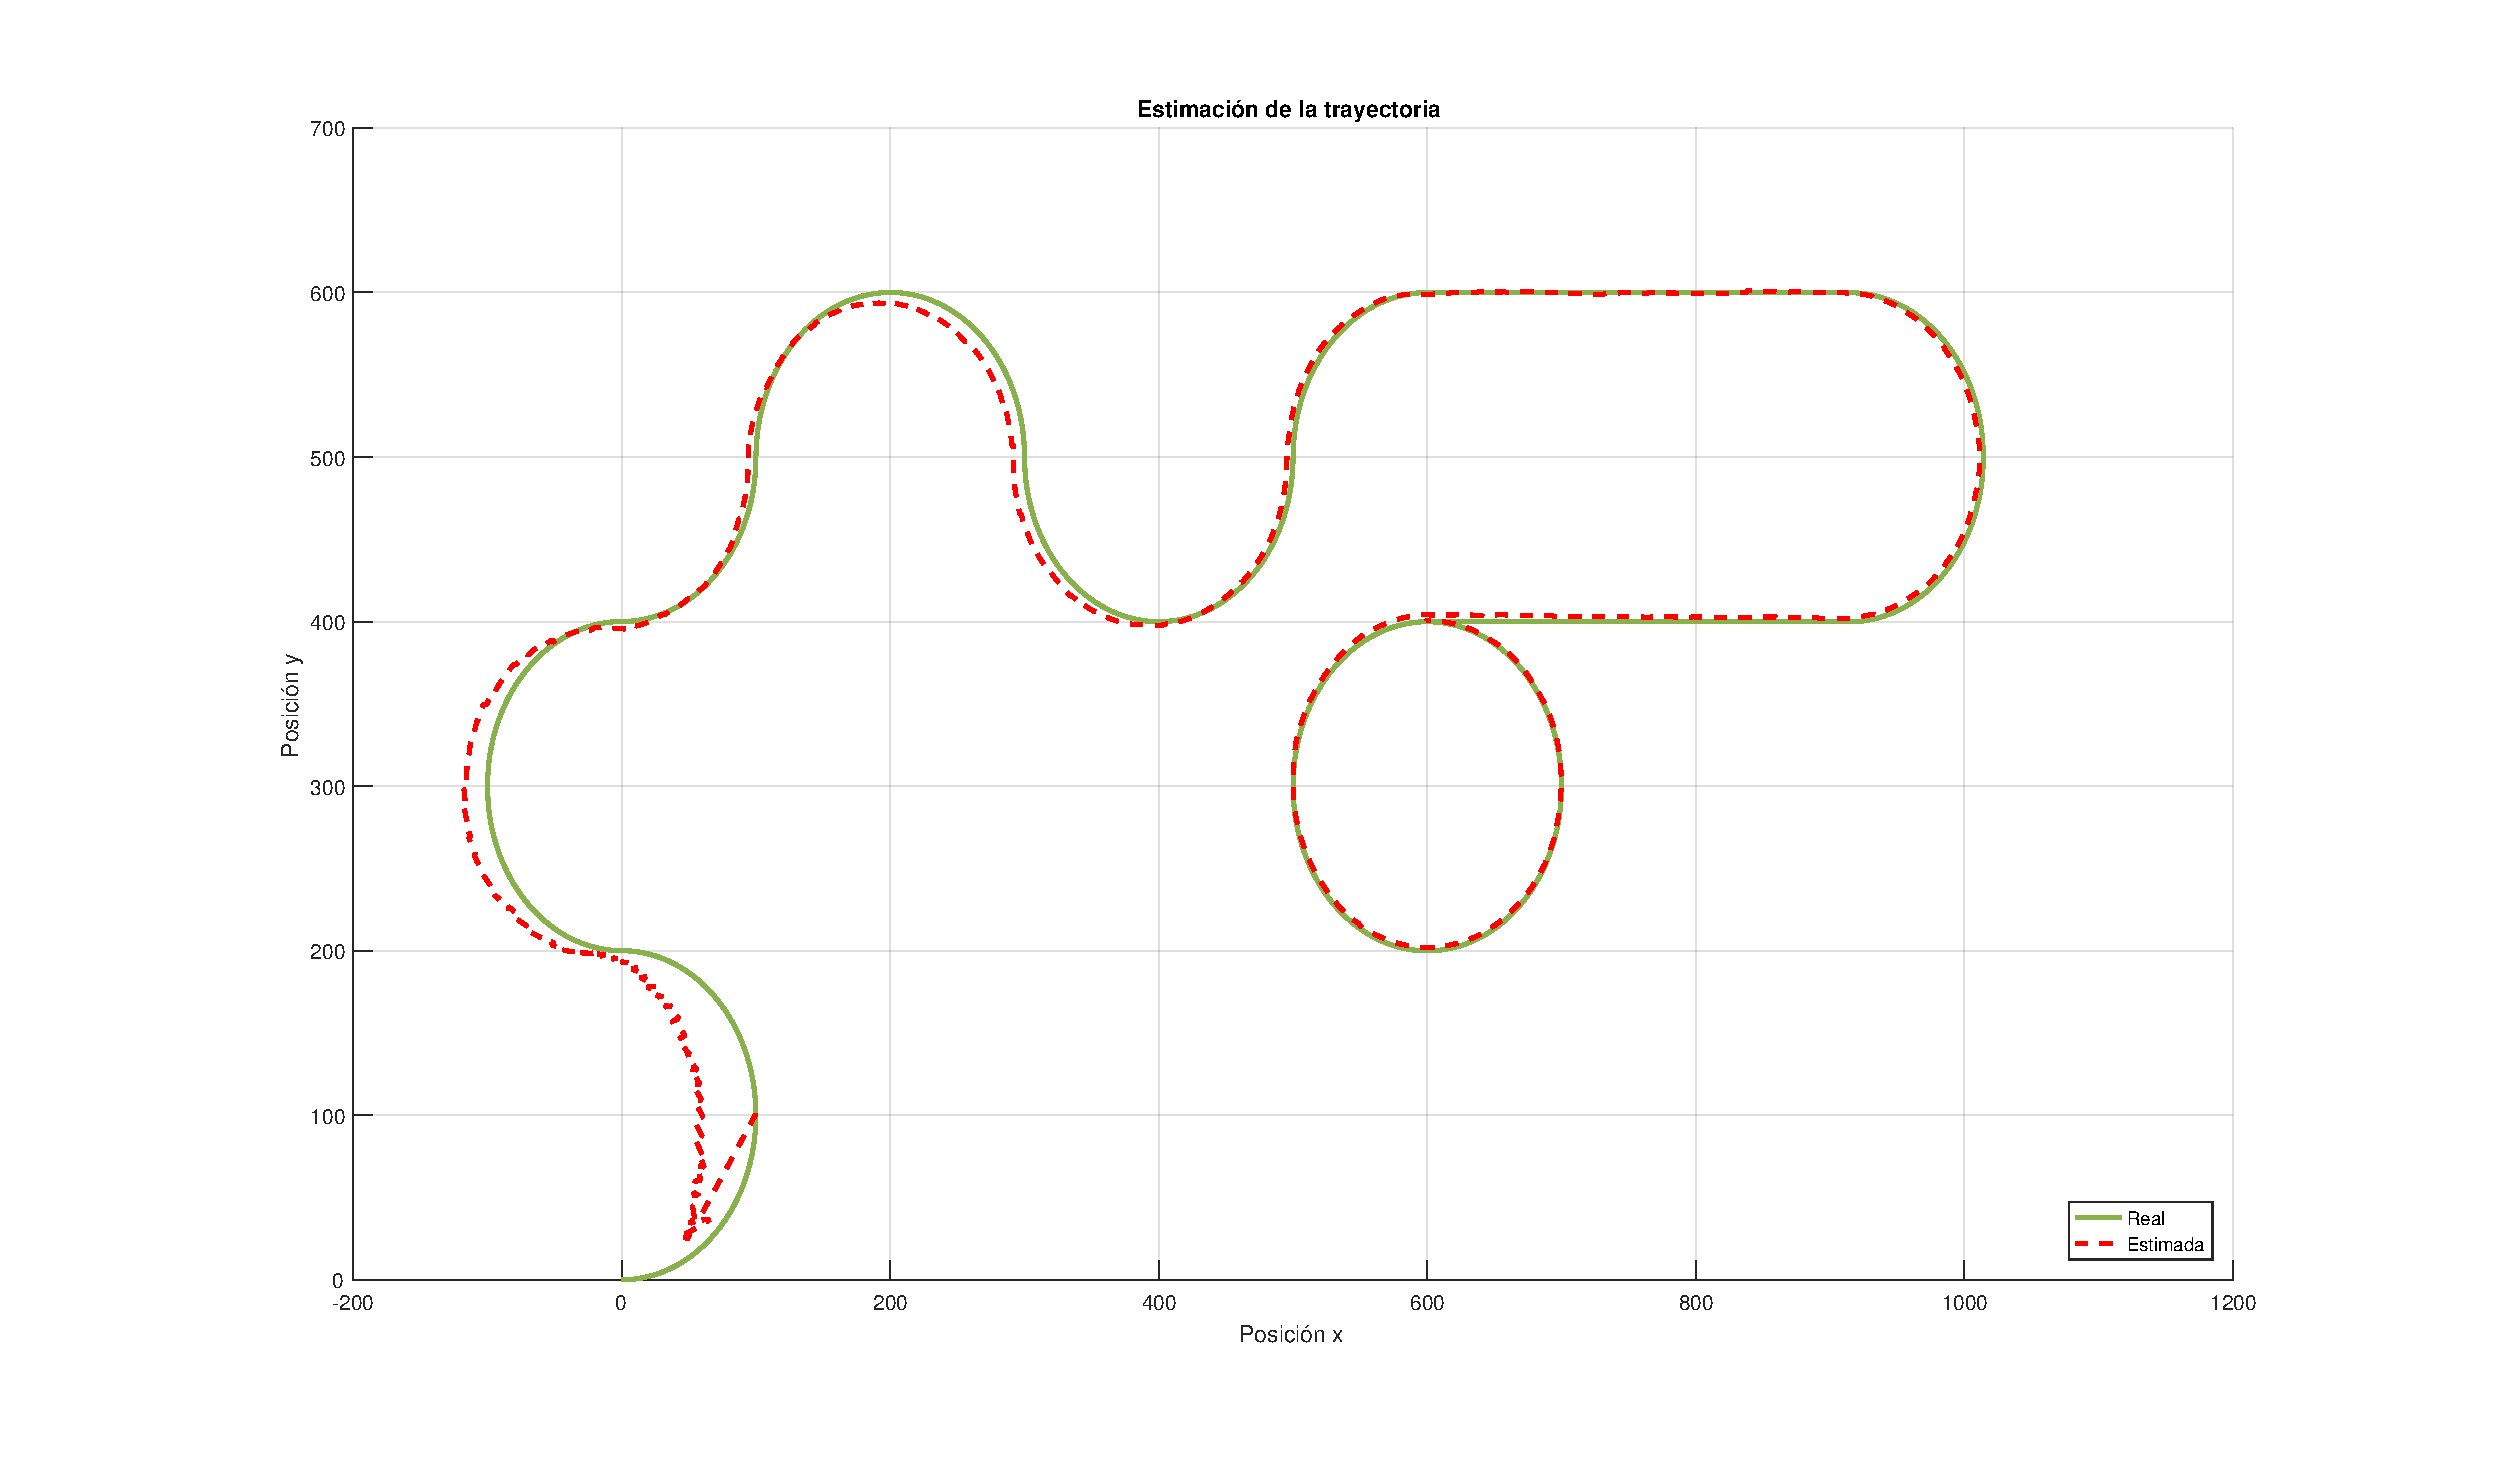
\includegraphics[width=\textwidth, trim= 2cm 2cm 2cm 2cm]{graf_ej3.pdf}
\caption{Estimación de la trayectoria.}
\label{fig:ej3} 
\end{figure}

	De la misma forma que en el trabajo previo, para la estimación del sesgo se lo agrega al vector de estados al sesgo en ambas coordenadas. Se supone que dicho sesgo es constante, por lo tanto la dinámica del mismo es constante y ruido de proceso nulo. Como el sesgo es en velocidad, a la matriz $C$ se le agregan 2 columnas cuyas dos últimas filas corresponden a la matriz identidad de $2\times 2$. Así las mediciones de velocidad tendrán adheridas los sesgos. Con lo expuesto, se obtiene la trayectoria de la Figura \ref{fig:ej3}. Realizando el test de observabilidad, se ve que todos los estados son observables. Viendo también las innovaciones en la Figura \ref{fig:3covinn} se confirma que las correlaciones son similares al de un proceso blanco asegurando que la estimación es correcta.\\ 

%\graficarPDF{graf_ej3_covinn}{Innovaciones de las posiciones y velocidades en $x^e$ e $y^e$.}{fig:3covinn}

\begin{figure}[H]
\centering
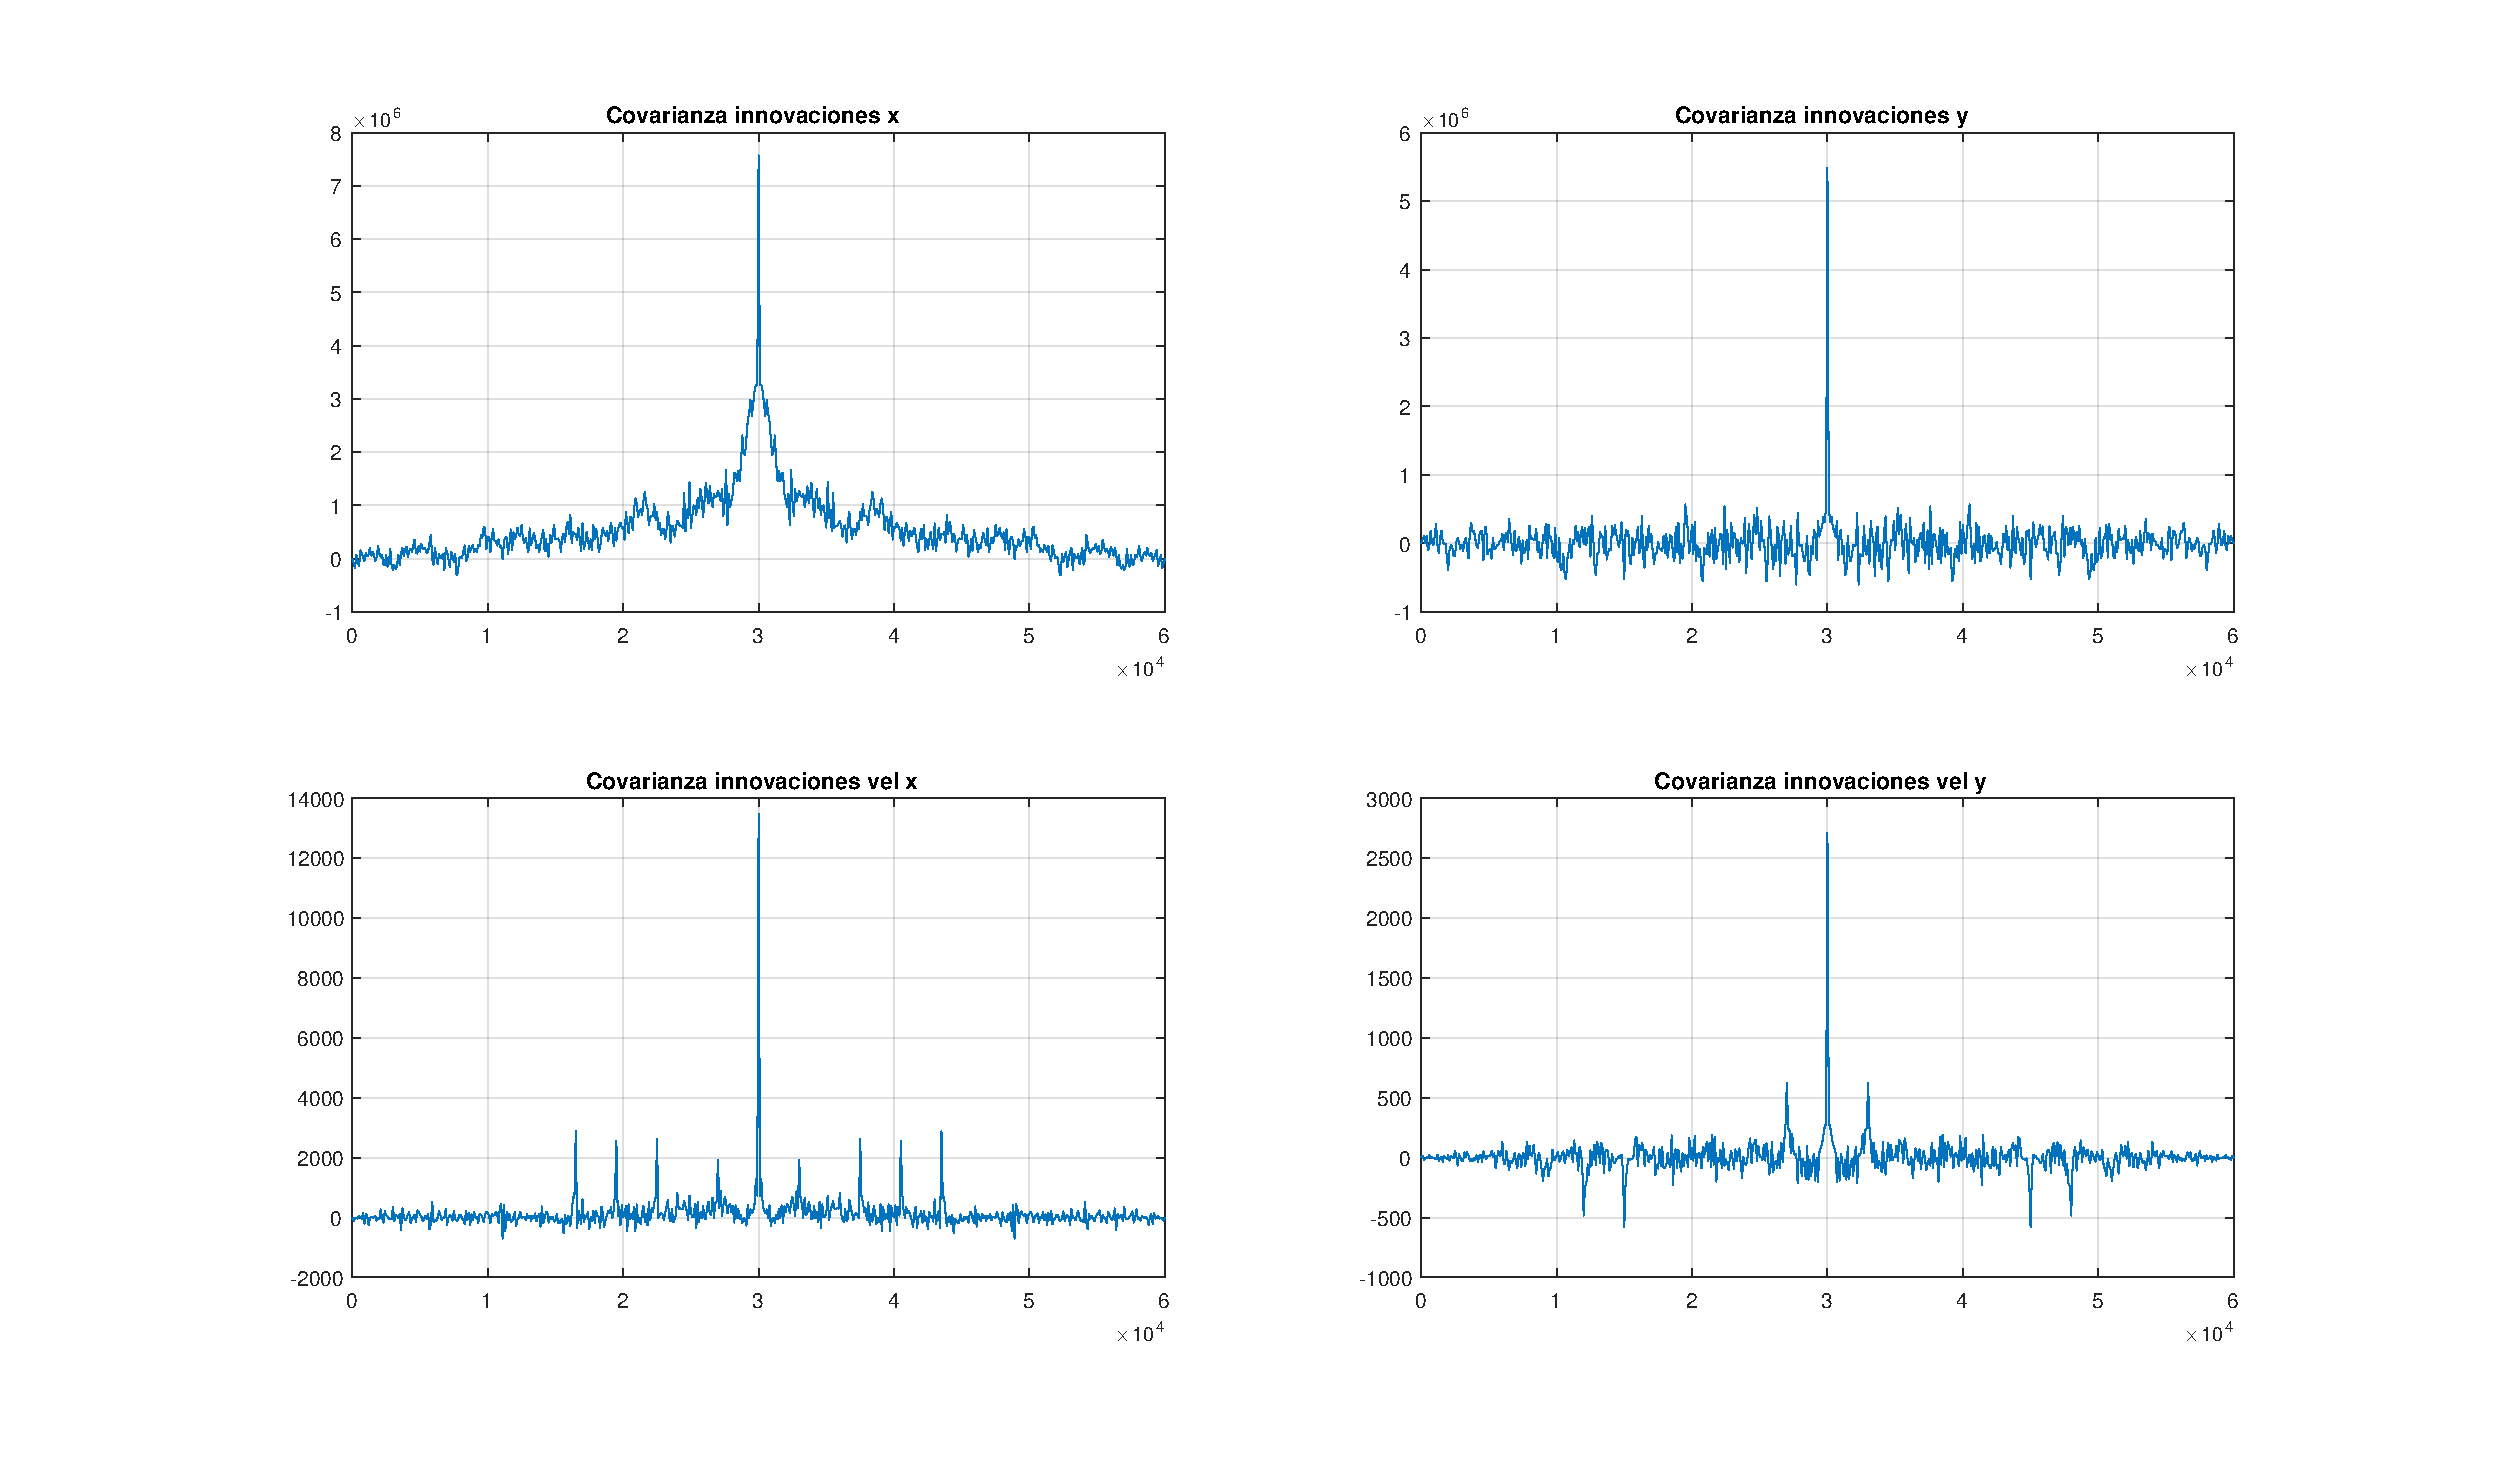
\includegraphics[width=0.9\textwidth,trim= 2cm 2cm 2cm 2cm]{graf_ej3_covinn.pdf}
\caption{Innovaciones de las posiciones y velocidades en $x^e$ e $y^e$.}
\label{fig:3covinn} 
\end{figure}

\pagebreak


%\graficarPDFa{0 05cm 0 13cm}{graf_ej3_pos}{Posición y error de la misma en función del tiempo.}{fig:3pos}

\vspace*{\fill}
\begin{figure}[H]
\centering
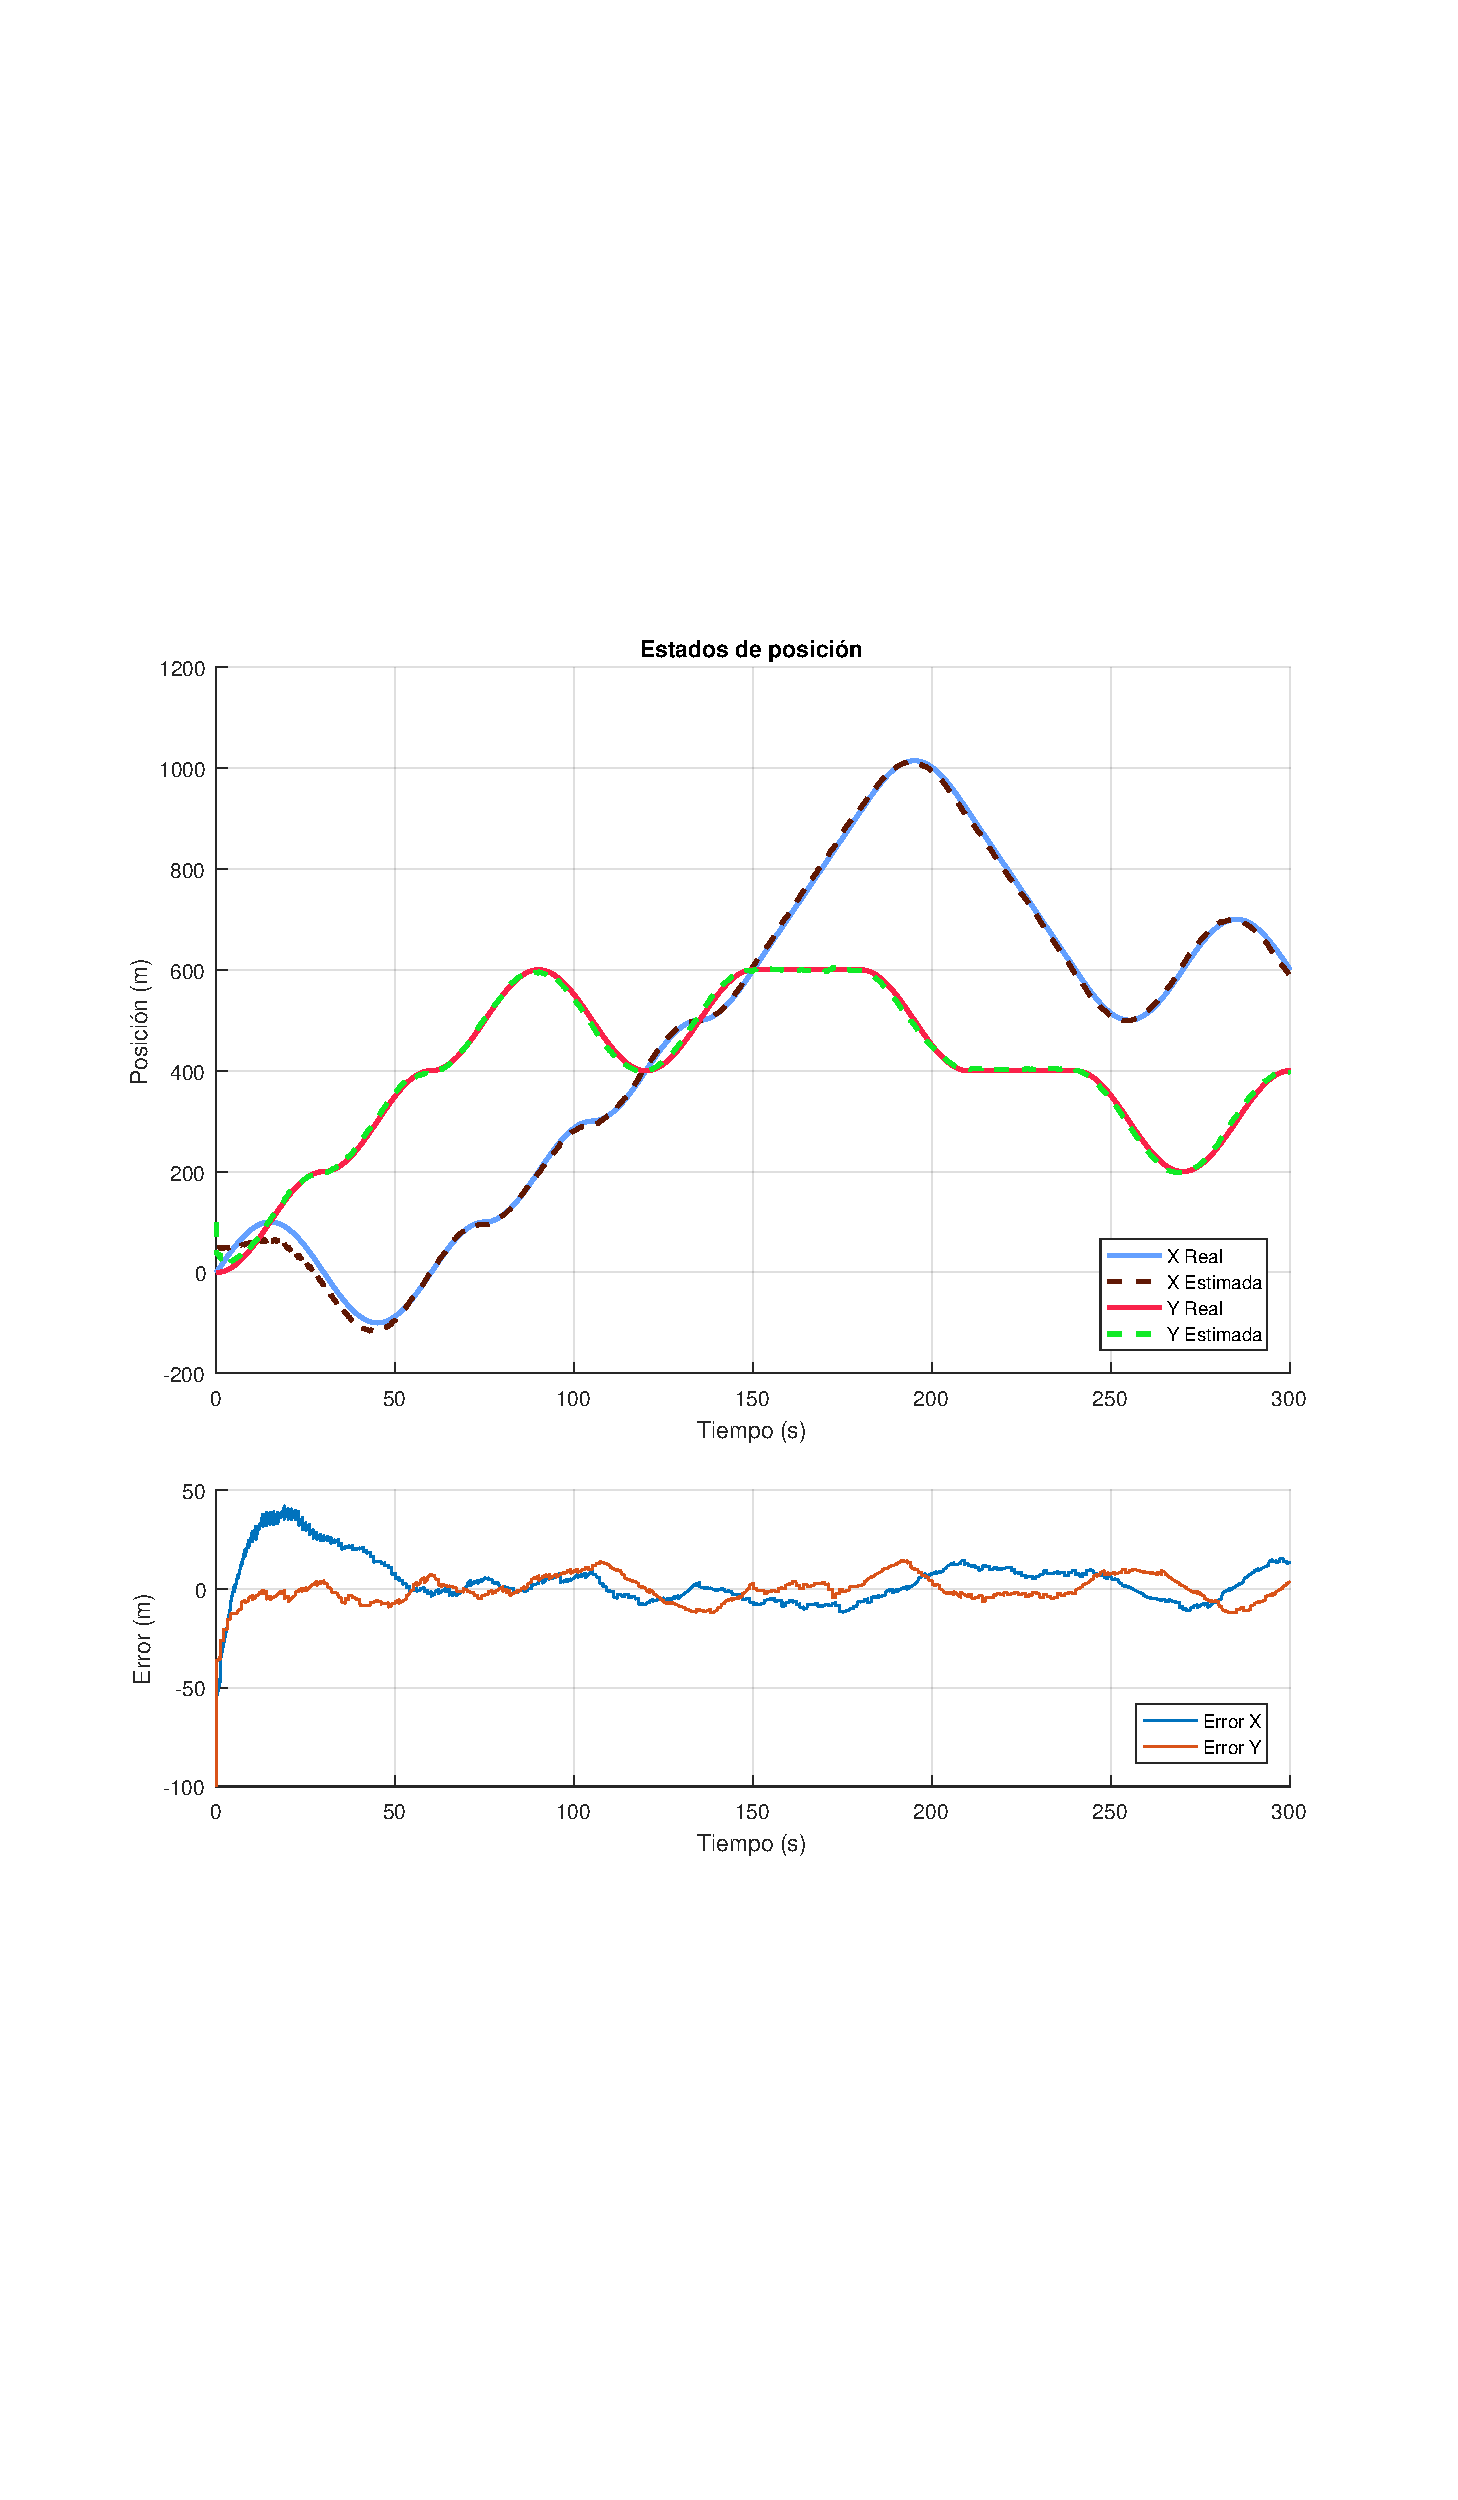
\includegraphics[scale=0.65, trim=6cm 6cm 6cm 6cm]{graf_ej3_pos.pdf}
\caption{Posición y error de la misma en función del tiempo.}
\label{fig:3pos} 
\end{figure}
\vspace*{\fill}

\pagebreak


%\graficarPDFa{0 05cm 0 15cm}{graf_ej3_vel}{Velocidad real y estimada en función del tiempo.}{fig:3vel}

\vspace*{\fill}
\begin{figure}[H]
\centering
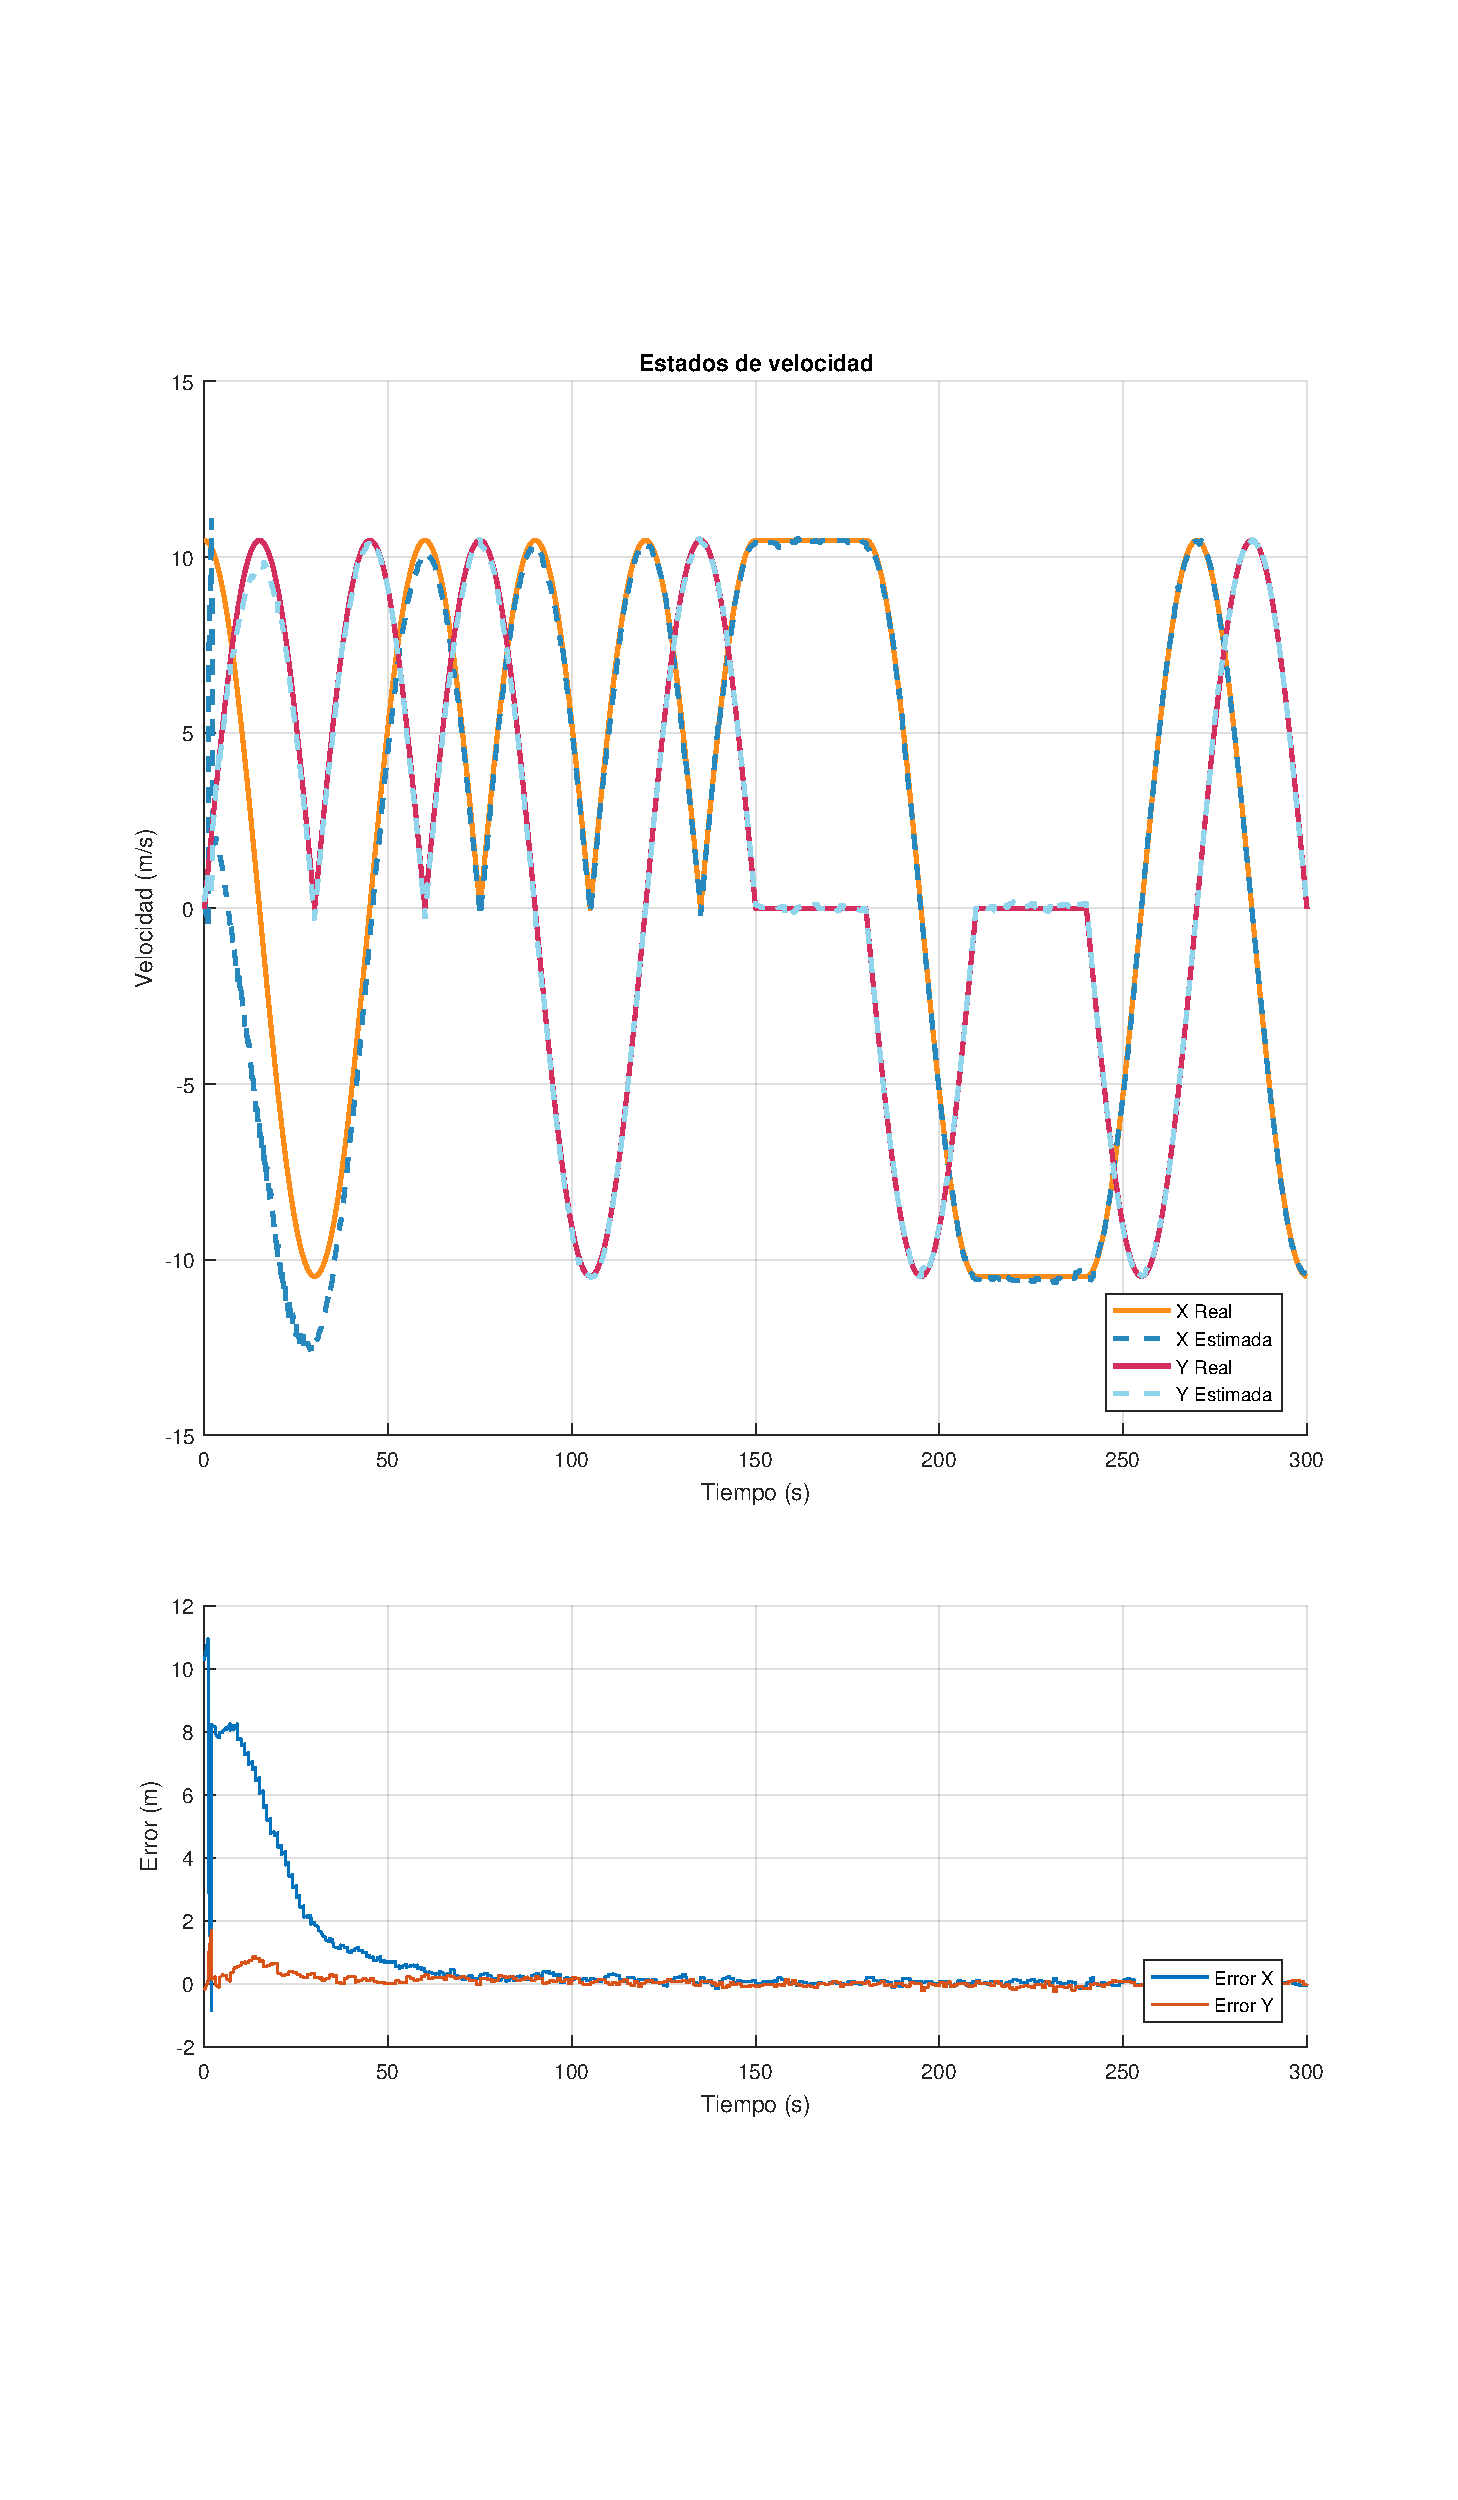
\includegraphics[scale=0.65, trim= 6cm 6cm 6cm 6cm]{graf_ej3_vel.pdf}
\caption{Velocidad real y estimada en función del tiempo.}
\label{fig:3vel} 
\end{figure}
\vspace*{\fill}

\pagebreak

\vspace*{\fill}
\graficarPDF{graf_ej3_theta}{Valores de los coeficientes de $C^e_b$ en el tiempo.}{fig:3theta}
\vspace*{\fill}

	\section{Estimación con sesgo en posición en el radar}\label{sec:ej4}
		
\graficarPDF{graf_ej4}{Estimación de la trayectoria.}{fig:ej4}
	El procedimiento para realizar la estimación con sesgo en posición es similar al punto anterior, a excepción de la matriz $C$ donde la identidad se encuentra ahora en las primeras 2 filas de las últimas 2 columnas. Como era de esperar por los resultados obtenidos en el trabajo anterior, no es posible la estimación de la trayectoria dado que los estados del sesgo no son observables. Es por tanto que se obtiene la estimación de la Figura \ref{fig:ej4} que sigue a la trayectoria pero con un \emph{offset} dado por el sesgo que no pudo ser estimado. Ésto se puede ver en el error en posición en la Figura \ref{fig:4pos}, siendo el mismo patrón que en el ejercicio \ref{sec:ej2} pero desplazado verticalmente.

%\graficarPDF{graf_ej4_covinn}{Innovaciones de las poisciones y velocidades en $x^e$ e $y^e$.}{fig:4covinn}

\begin{figure}[H]
\centering
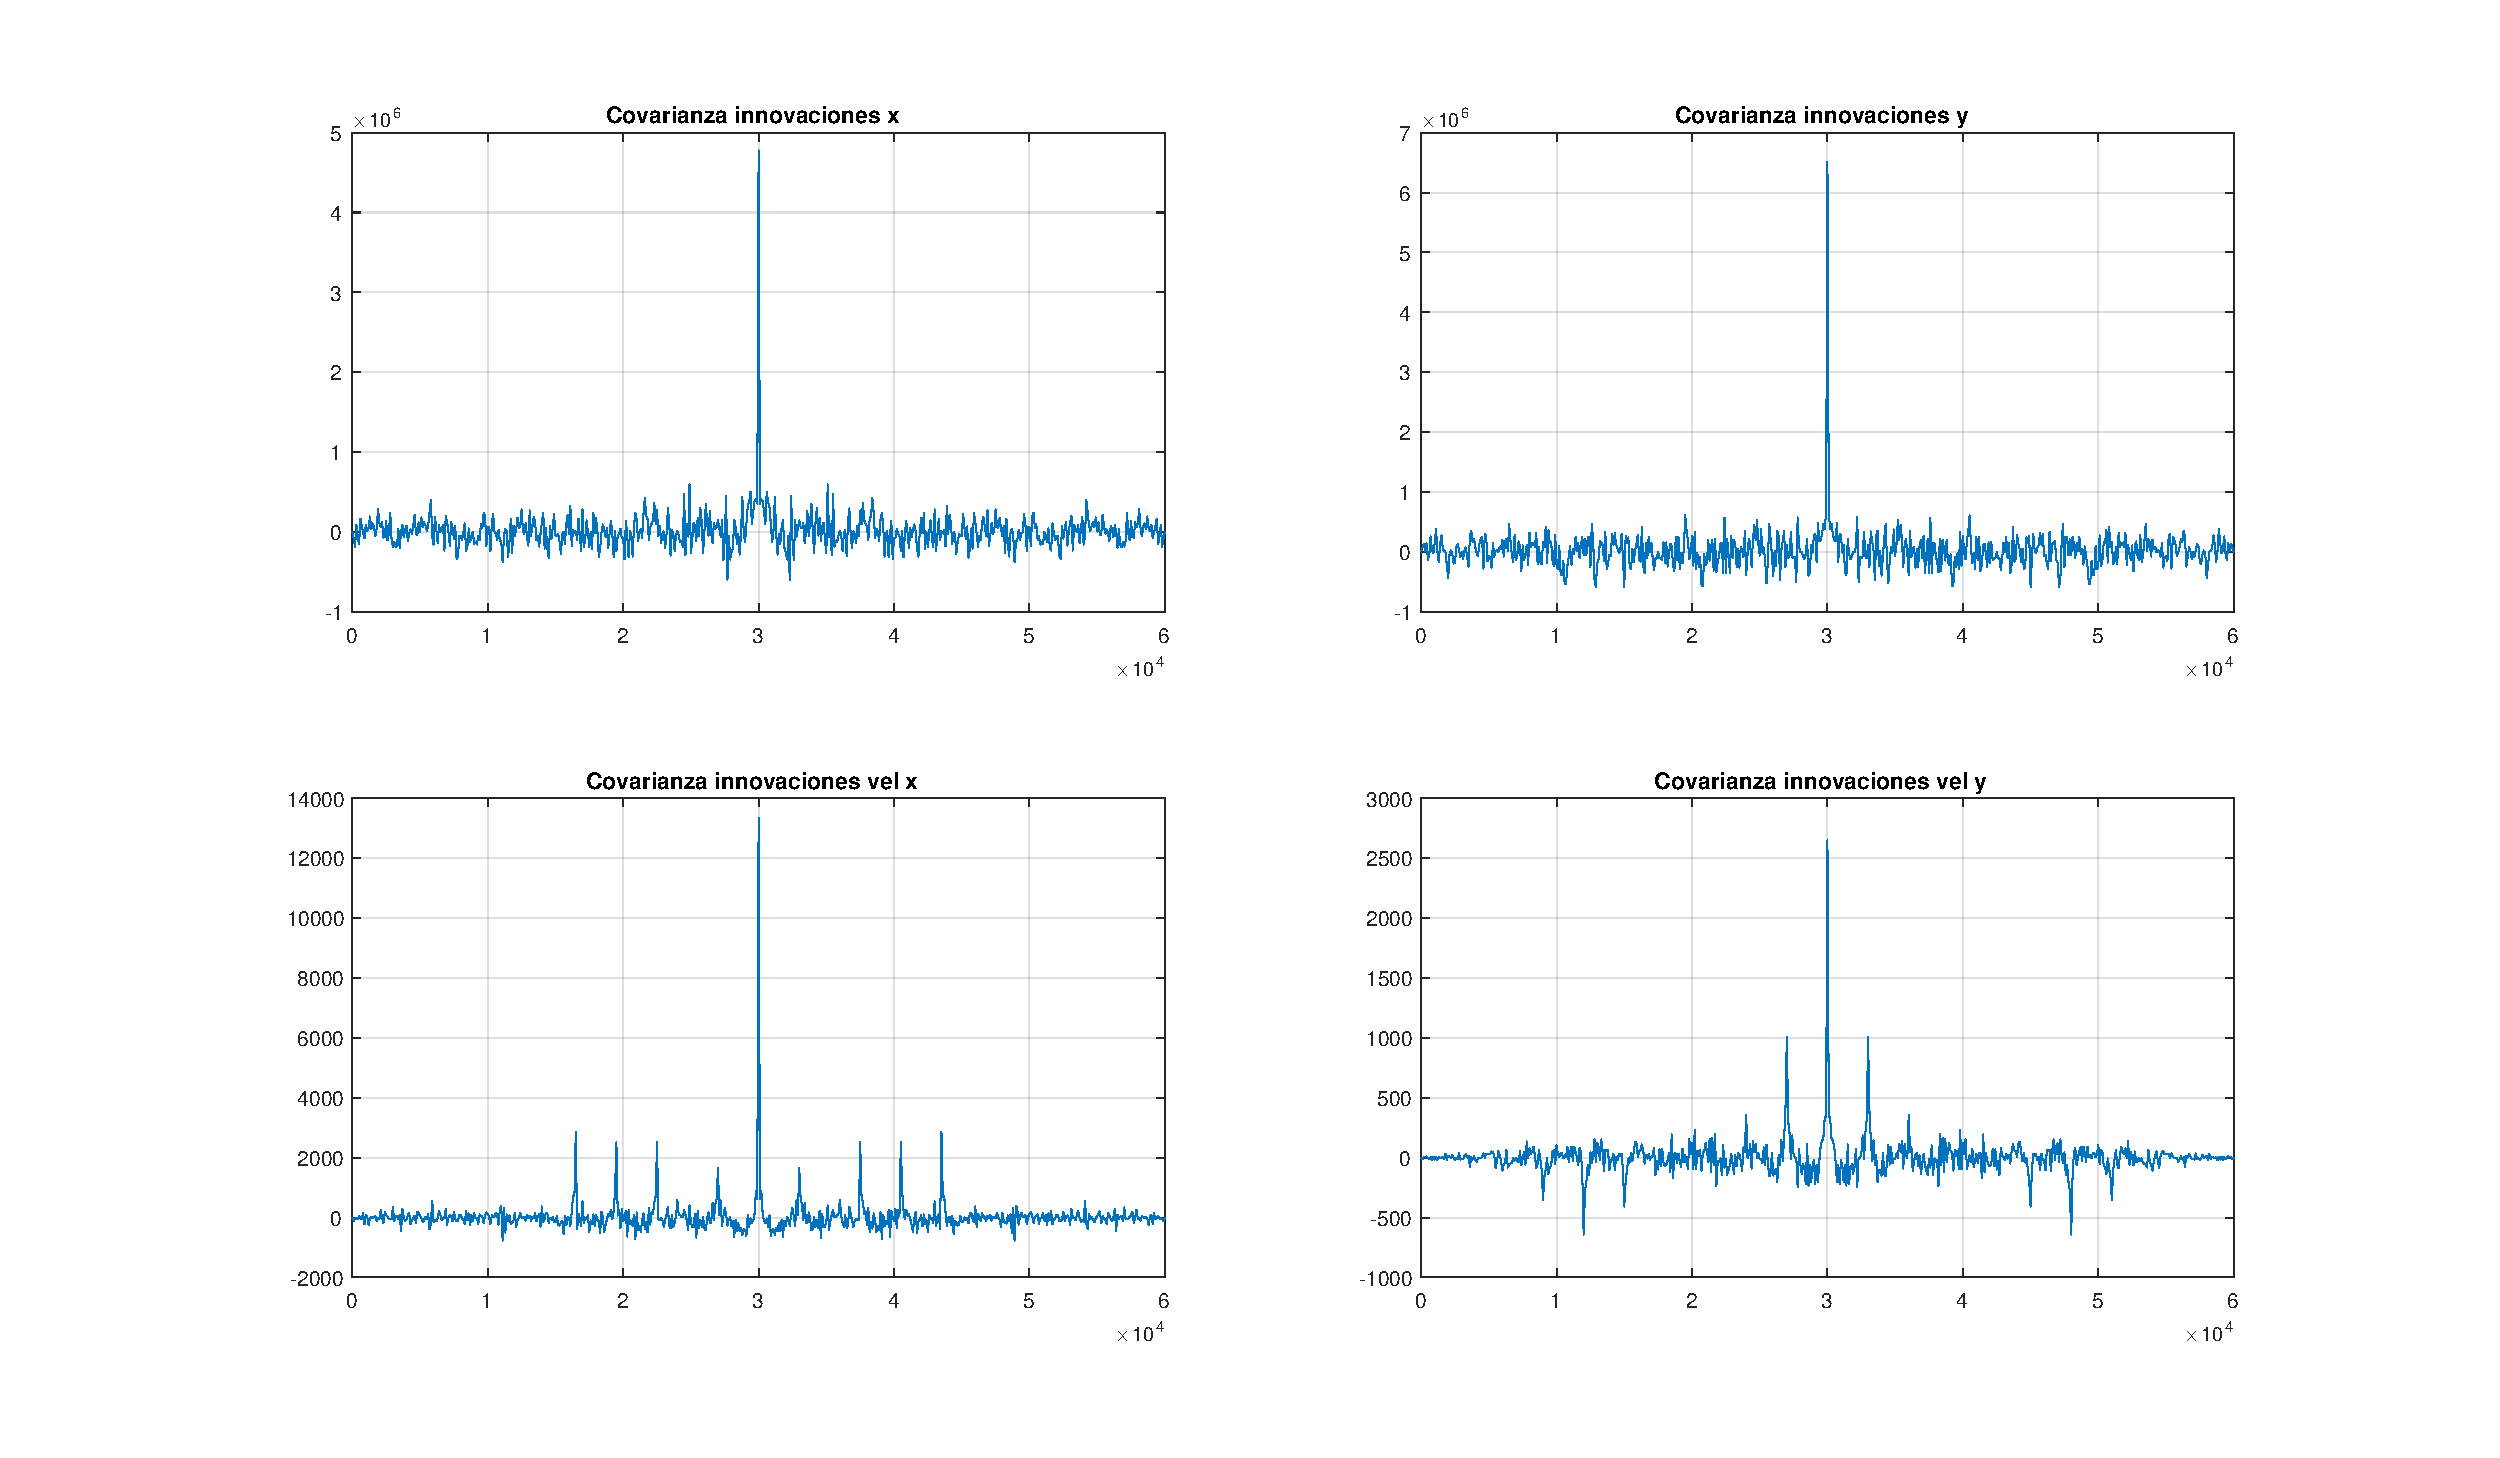
\includegraphics[width=0.9\textwidth,trim= 2cm 2cm 2cm 2cm]{graf_ej4_covinn.pdf}
\caption{Innovaciones de las posiciones y velocidades en $x^e$ e $y^e$.}
\label{fig:4covinn} 
\end{figure}


\pagebreak

%\graficarPDFa{0 10cm 0 10cm}{graf_ej4_pos}{Posición ej4}{fig:4pos}

\vspace*{\fill}
\begin{figure}[H]
\centering
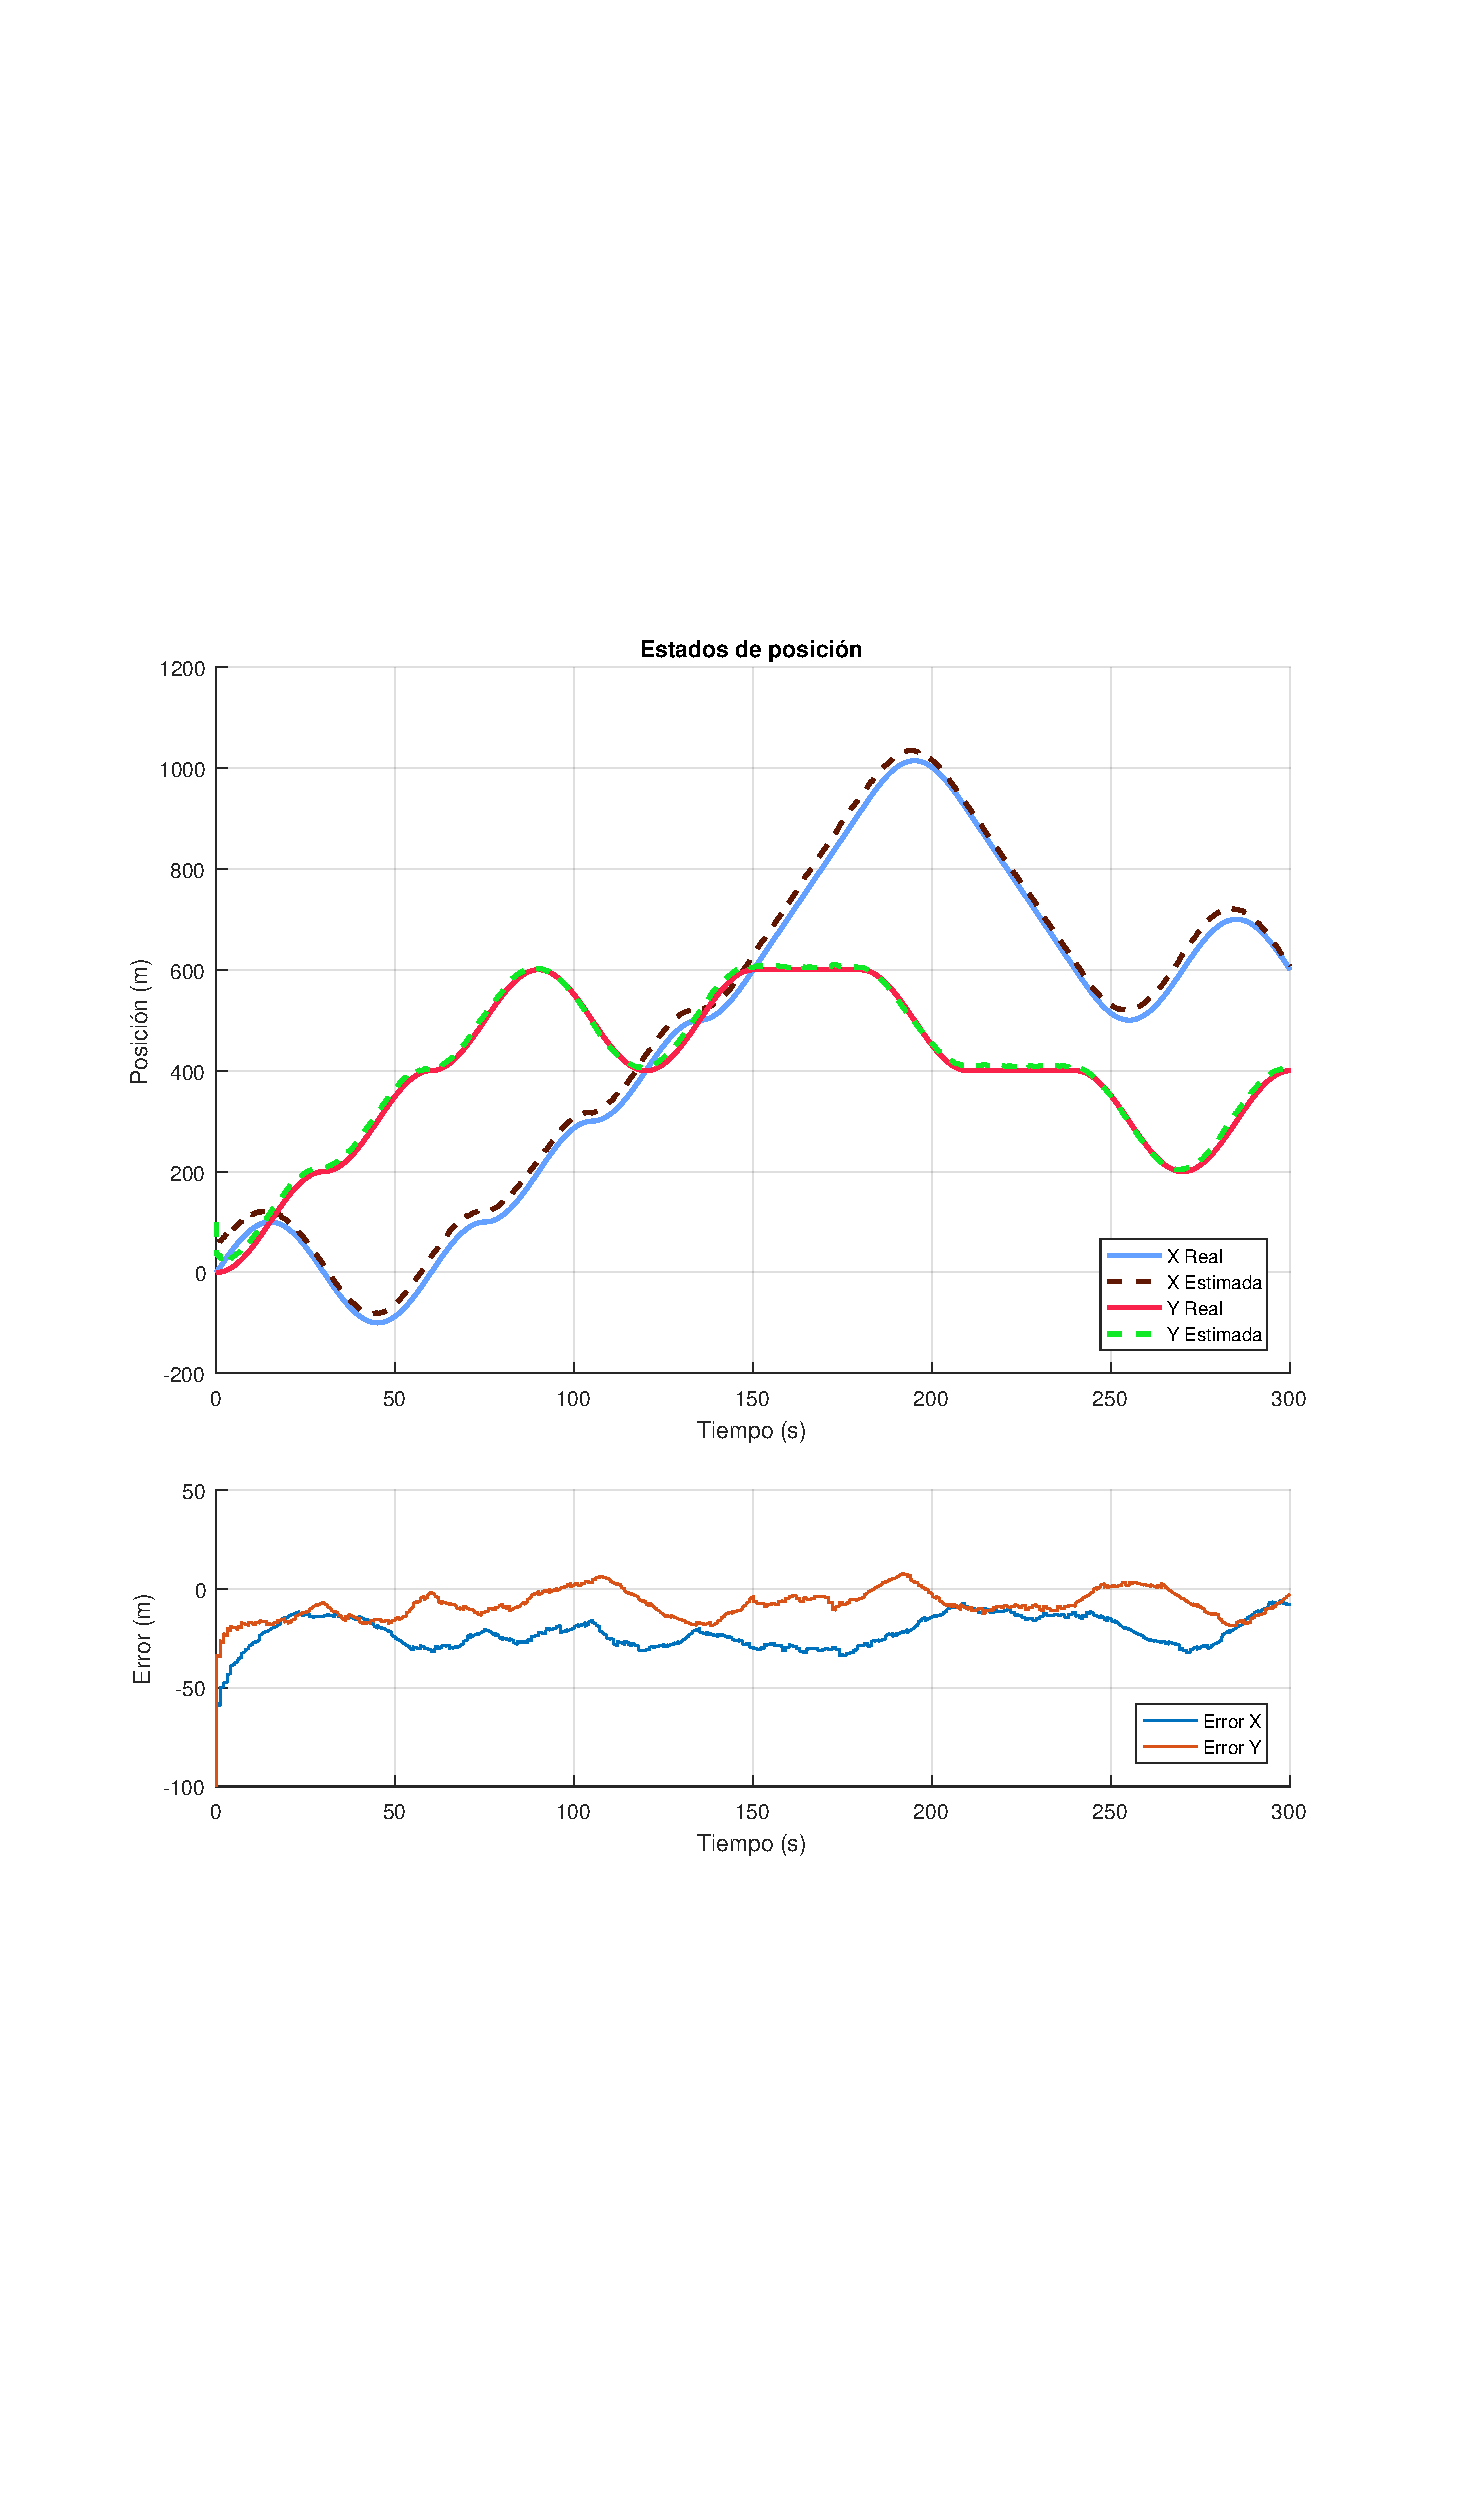
\includegraphics[scale=0.5, trim= 6cm 6cm 6cm 6cm]{graf_ej4_pos.pdf}
\caption{Posición y error en función del tiempo.}
\label{fig:4pos} 
\end{figure}
\vspace*{\fill}

\pagebreak

%\graficarPDFa{0 10cm 0 10cm}{graf_ej4_vel}{Velocidad real y estimada en función del tiempo.}{fig:4vel}

\vspace*{\fill}
\begin{figure}[H]
\centering
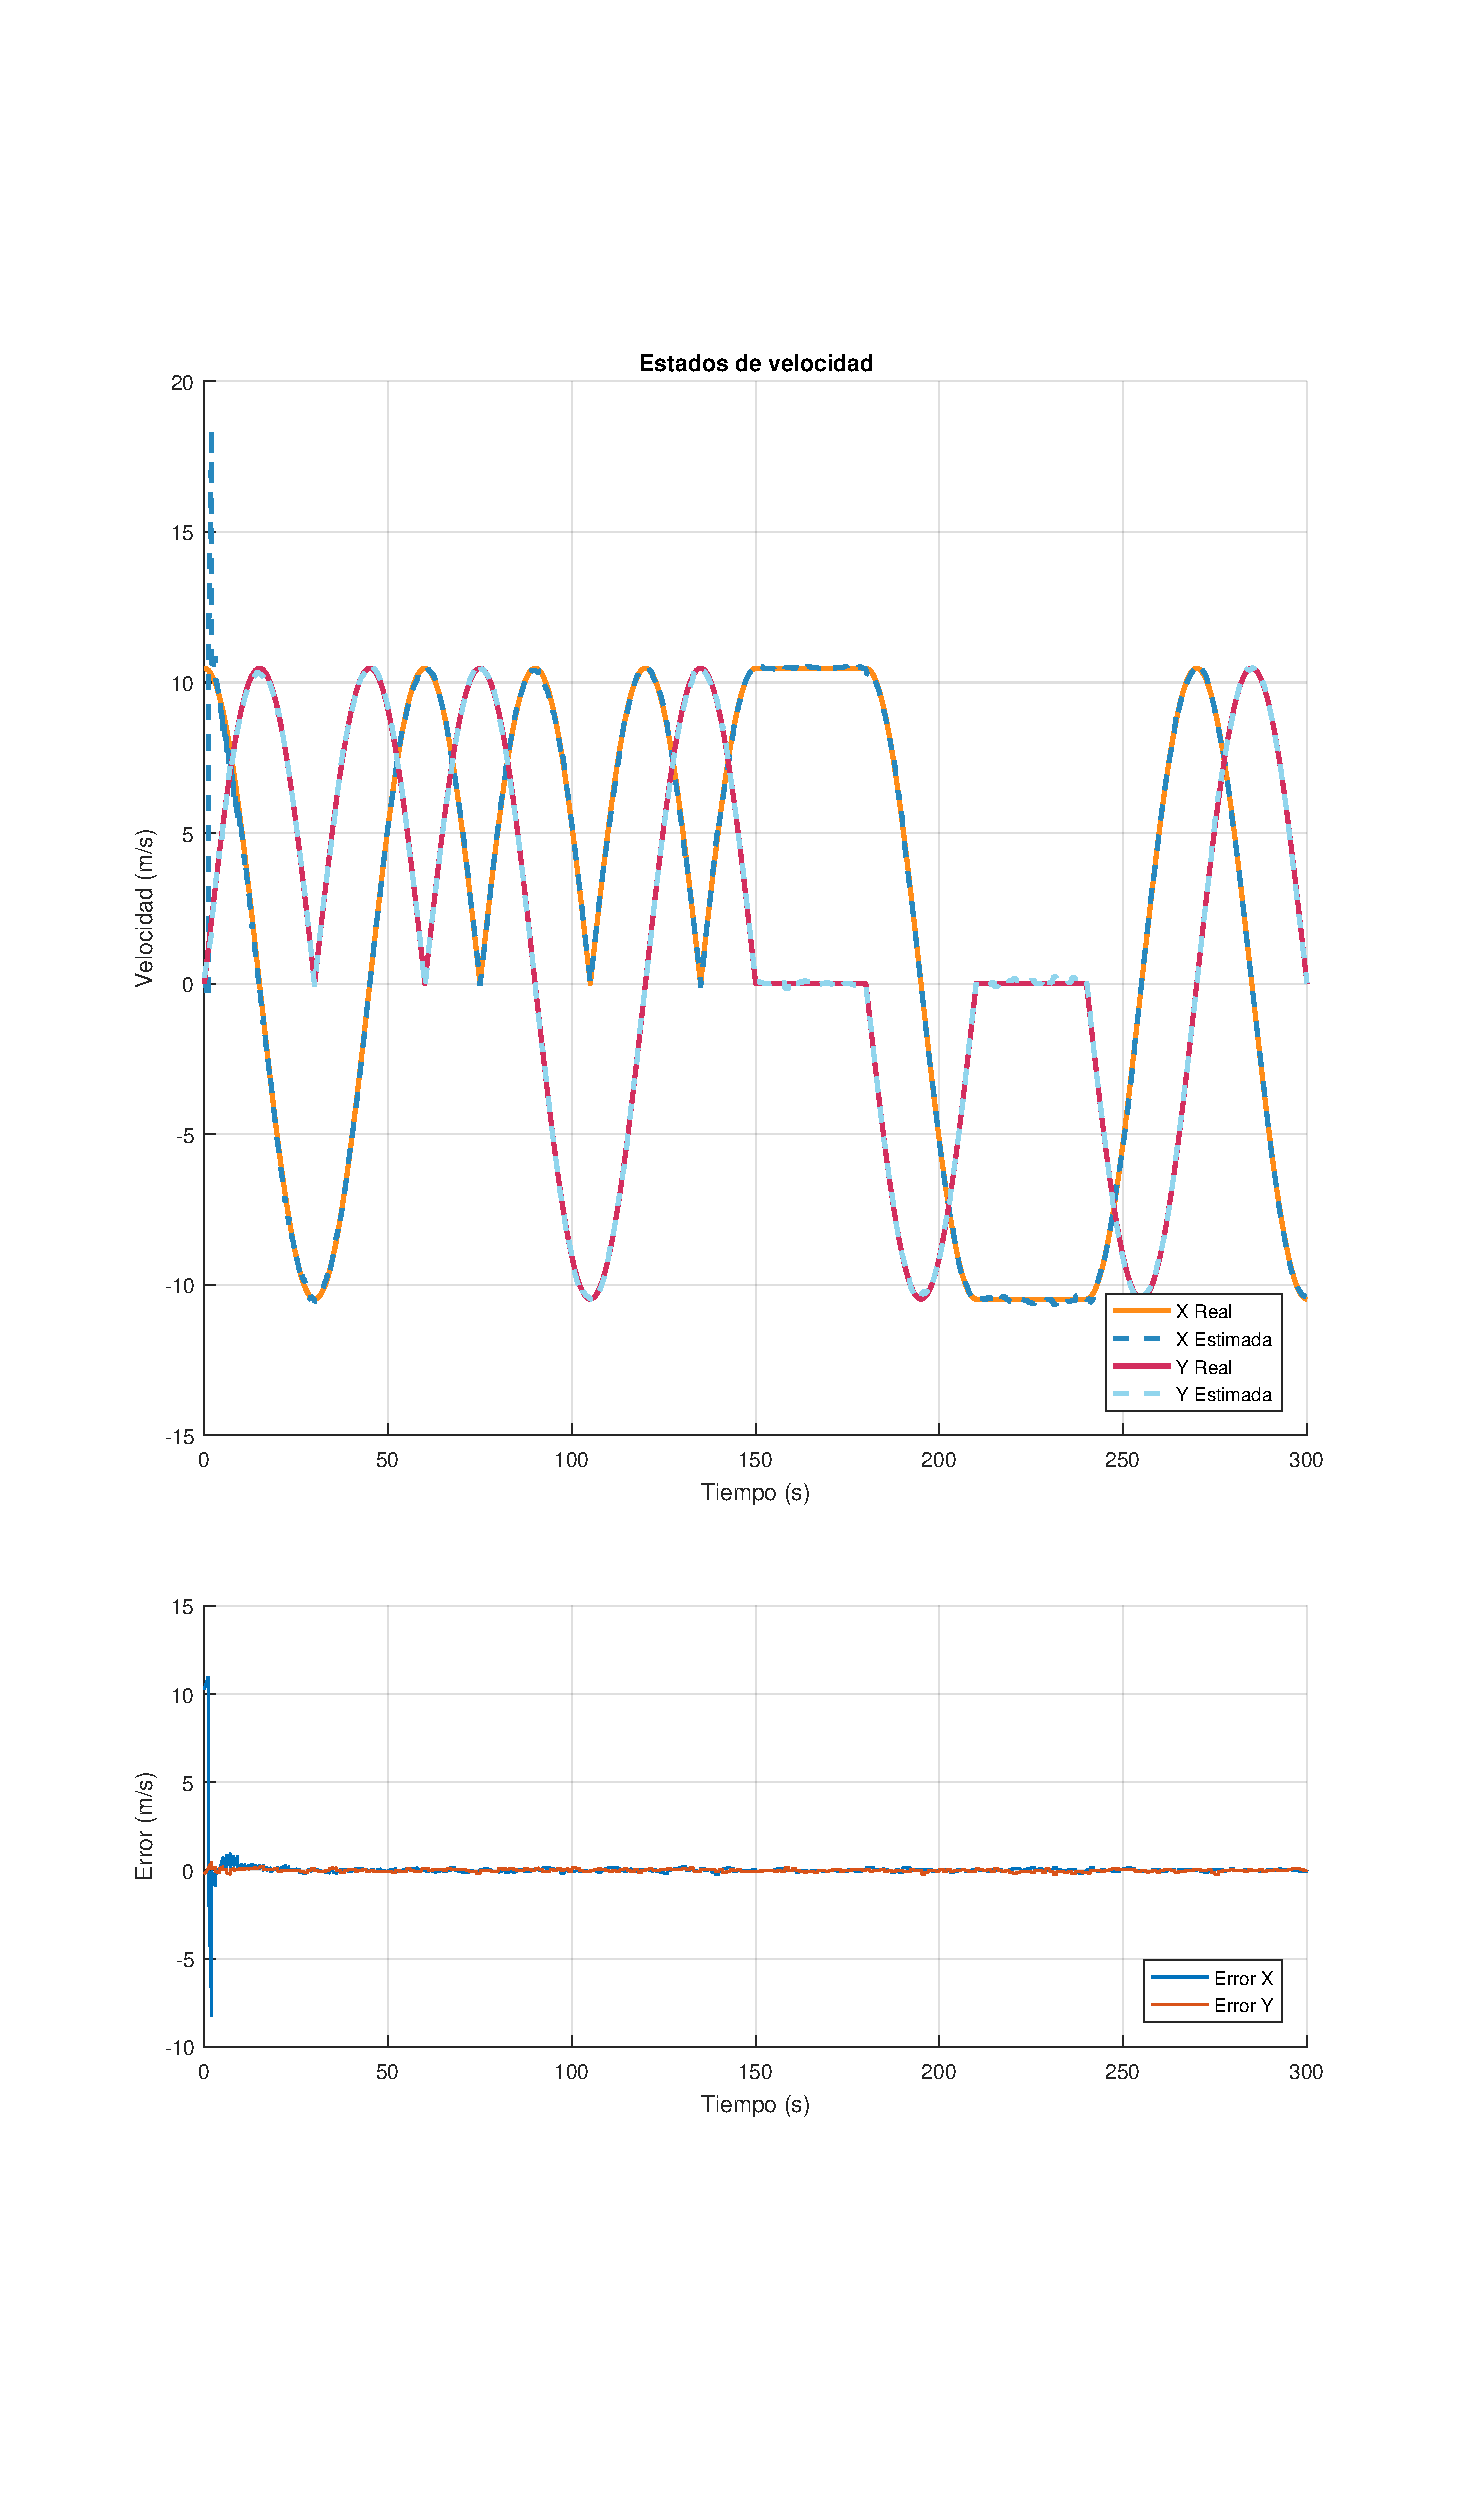
\includegraphics[scale=0.5, trim= 5cm 5cm 5cm 5cm]{graf_ej4_vel.pdf}
\caption{Velocidad real y estimada en función del tiempo.}
\label{fig:4vel} 
\end{figure}
\vspace*{\fill}


\pagebreak
\graficarPDF{graf_ej4_theta}{Valores de los coeficientes de $C^e_b$ en el tiempo.}{fig:4theta}



	\section{Filtro de Kalman con factorización QR y de Cholesky}\label{sec:ej5}
			
	Se define la descomposición de \emph{Cholesky} como la matriz $X^{c}_k$ tal que:
	\begin{equation*}
		X_k = X^{c^{H}}_k X^{c}_k
	\end{equation*}	

	A partir de ello, se propone para el filtro de Kalman definir: 
	\begin{equation*}
		M_0 = \begin{bmatrix} R^{c}_k& C_k\; P^c_{k/k-1}& 0 \\[0.3em] 0& A_k\; P^c_{k/k-1}& B_k\; Q^c_k \end{bmatrix}
	\end{equation*}
	de modo que al factorizar $M^H_0 = Q\,R$ se obtiene que $A=R^H R$, es decir que $R$ es la factorización de \emph{Cholesky} de $A$. Para optimizar los cálculos, se le agrega una fila a dicha matriz para incorporar las mediciones. Entonces:
	\begin{equation*}
	M =  \begin{bmatrix} R^{c}_k& C_k\; P^c_{k/k-1}& 0 \\[0.3em] 0& A_k\; P^c_{k/k-1}& B_k\; Q^c_k \\[0.3em] -y^H\,R^{c^{-1}}_k & \hat{x}^H\, P^{c^{-1}}_{k/k-1} & 0 \end{bmatrix}
	\end{equation*}

	Como la matriz $R$ será triangular inferior (propiedad de la factorización \emph{QR}) se tiene:
	\begin{equation*}
	R^H = \begin{bmatrix} X&0&0\\[0.3em]Y&Z&0\\[0.3em]W_1&W_2&W_3\end{bmatrix} \text{ donde } \begin{cases} P_{k+1/k} = Z\,Z^H\\ \hat{x}_{k+1/k}=Z\,W^H_2\\ \hat{g}_k = -X\,W^H_1\end{cases}
	\end{equation*}



	\section{Verificación de los resultados del filtro de Kalman}\label{sec:ej6}
			
	Para verificar si el filtro de Kalman está funcionando correctamente, se debe inspeccionar la correlación de las innovaciones. Las innovaciones constan de la parte ortogonal de las mediciones con la predicción de los estados. Cuanto más descorrelacionadas estén las innovaciones, mejor será la estimación dado que los datos que van arribando son útiles. De este modo, si la correlación de las innovaciones se asemeja al de un proceso blanco se puede afirmar que el algoritmo de Kalman estima correctamente.

	Por otro lado, deberá tenerse en cuenta la observabilidad del sistema porque las innovaciones pueden ser un proceso blanco pero si los estados no son observables, la estimación no será satisfactoria.


	\section{Estimación por Filtro de Kalman Extendido}\label{sec:ej7}
		
\graficarPDF{graf_ej7}{Estimación de la trayectoria.}{fig:ej7}
\graficarPDF{graf_ej7_covinn}{Innovaciones de las posiciones y velocidades en $x^e$ e $y^e$.}{fig:7covinn}
\graficarPDFa{0 10cm 0 10cm}{graf_ej7_pos}{Posición y error de la misma en función del tiempo.}{fig:7pos}
\graficarPDF{graf_ej7_theta}{Valores de los coeficientes de $C^e_b$ en el tiempo.}{fig:7theta}
\graficarPDF{graf_ej7_vel}{Velocidad real y estimada en función del tiempo.}{fig:7vel}
\graficarPDF{graf_ej7_sesgo}{Valores de los últimos \SI{100}{\s} del sesgo y su convergencia al valor real.}{fig:7sesgo}


%	\section{Conclusiones}\label{sec:conclusiones}
%		
	Tendría que chamuyar acá pero creo que los gráficos no están ajustando bien (fijarse en el tp de Sampayo que da mucho mejor el error). No sé por qué es que sucede esto aún. Podríamos mandarle el código de Débora para que le pegue una ojeada (que además ella quería que se lo mandemos). En realidad yo estoy para mandarle el repositorio entero con el pdf adjunto para que vaya leyendo y nos haga una precorrección.\\
	\indent Otra cosa copada que dijo mariano que podríamos hacer es, en lo que da mal, agregar la variación de la varianza en función del tiempo. Ahí veríamos si el problema del error es de ahí o algo más.


	% \appendix
\end{document}
